\documentclass[
	ngerman,
% 	english,
	10pt,				% Schriftgröße anpassen, Standard ist 11pt, nicht weniger als 8pt verwenden!
	aspectratio=169 	% für 16:9 Format
]{beamer}


% \includeonlyframes{erk8,zf1}
\newsavebox{\mysaveboxa}
\newsavebox{\mysaveboxb}
\usepackage{lmodern}

\synctex=1
\usepackage[utf8]{luainputenc}
\usepackage[TS1,T1]{fontenc}
\usepackage{babel}
\usepackage{biblatex}
\usepackage[absolute,overlay]{textpos} % für \textblock
\usepackage{tcolorbox}
\usepackage{listings}
\usepackage{stmaryrd} % for \lightning


\usepackage{xcolor}
\newcommand{\tcblue}[1]{\textcolor{blue}{#1}} % für tmp-Hervorhebungen





% https://tex.stackexchange.com/questions/101858/make-two-figures-aligned-at-top
\usepackage[export]{adjustbox} % für "vertical alignment"



\usepackage{tikz}

\usetikzlibrary{decorations.pathreplacing}

\newcommand*\circledz[1]{\tikz[baseline=(char.base)]{
            \node[shape=circle,draw,inner sep=2pt] (char) {#1};}}



\newcommand*\circled[1]{\scalebox{0.7}{\tikz[baseline=(char.base)]{
            \node[shape=circle,draw,inner sep=2pt] (char) {#1};}}}


% Thema festlegen
\usetheme[
	pagenum,
	%ddc,		% Dresden concept Logo einbinden
	serifmath,	% vernünftige Schriftart für Formeln
]{tud}


% bib-Datei mit den Literaturangaben
% ==================================
% \addbibresource{Literatur.bib}


% allgemeine Angaben
% ==================
\title[Modellbildung und Reglerentwurf Brückenkransystem]{Verteidigung der Studienarbeit: Modellbildung und Reglerentwurf für ein Brückenkransystem}
\subtitle{}

\author{Konstantin Wrede}
\datecity{Dresden}
\date{XX. November 2022}


% Angaben zum Institut usw.
% =========================
% entweder
	%\institute{}
% oder
	\einrichtung{TU Dresden}
	%\fachrichtung{Fachrichtung}
	\institut{Institut für Regelungs- und Steuerungstheorie}
%	\professur{Professur}


% Anpassung des äußeren Erscheinungsbildes
% ========================================
% RST-Logo als Zweitlogo
\setbeamertemplate{zweitlogo/titlepage}[logofile]{img/Logo-RST-HKS41.pdf}
% Aktivieren der Folie vor jeder Section (nicht vor \section*)
\AtBeginSection[]{\partpage{\usebeamertemplate***{part page}}}


% für extra/folien backup-slides

\newcommand{\backupbegin}{
   \newcounter{finalframe}
   \setcounter{finalframe}{\value{framenumber}}
}
\newcommand{\backupend}{
   \setcounter{framenumber}{\value{finalframe}}
}


% Anpassung des Layouts
% =====================
% Abstand vor und nach Formeln festlegen
\setlength\abovedisplayshortskip{0pt}
\setlength\belowdisplayshortskip{3pt}
\setlength\abovedisplayskip{5pt}
\setlength\belowdisplayskip{5pt}



% aus der Diss-Verteidigung

\definecolor{tublue}{rgb}{0.14, 0.25, 0.38}
\definecolor{tubluee}{rgb}{0.95, 0.96, 0.99}
\definecolor{myred}{rgb}{0.73,0.10,0.10}
\definecolor{myorange}{rgb}{0.85,0.45,0.10}
\definecolor{mygreen}{rgb}{0.10,0.6,0.10}
\definecolor{myblue}{rgb}{0.2,0.25,0.7}
\definecolor{mygray}{rgb}{0.7,0.7,0.7}

\definecolor{tublue}{rgb}{0.14, 0.25, 0.38}
\definecolor{tubluee}{rgb}{0.95, 0.96, 0.99}

\definecolor{softblue}{rgb}{0.3,0.3,.6}
\definecolor{lightblue}{rgb}{0.9,0.9,.95}


% \newcommand{\igrau}{\color{grau}}
\newcommand{\myemph}[1]{\textcolor{darkblue}{#1}}
\newcommand{\tcw}[1]{\textcolor{white}{#1}}
% \newcommand{\tcb}[1]{\textcolor{darkblue}{#1}}
\newcommand{\tcb}[1]{\textcolor{myblue}{#1}}
% \newcommand{\tcg}[1]{\textcolor{darkgreen}{#1}}
\newcommand{\tcg}[1]{\textcolor{mygreen}{#1}}
\newcommand{\ccg}[2]{{\color<#1>{mygreen}#2}}
\newcommand{\ccb}[2]{{\color<#1>{myblue}#2}}
% \newcommand{\tcr}[1]{\textcolor{brownz}{#1}}
\newcommand{\tcr}[1]{\textcolor{myred}{#1}}
\newcommand{\tcred}[1]{\textcolor{red}{#1}}
\newcommand{\tca}[1]{\textcolor{mygray}{#1}}


\newcommand{\cdbox}{$\square$\hspace{-0.65em}\raisebox{0.1em}{\checkmark}\hspace{-0.18em}}



\lstdefinelanguage{yaml}{
  keywords={true,false,null},
  keywordstyle=\color{green}\slshape,
  ndkeywords={type,types,params,methods,inputs,outputs,tune,unset,start,target},
  ndkeywordstyle=\color{blue}\bfseries,
  identifierstyle=\color{black},
  sensitive=false,
  %moredelim=[l]{}{:},
  comment=[l]{\#},
  morecomment=[s]{/*}{*/},
  commentstyle=\color{purple}\ttfamily,
  stringstyle=\color{blue}\ttfamily,
  %morestring=[l]{-}{},
  morestring=[b]',
  morestring=[b]"
}




\lstdefinelanguage{owlms}{
  keywords={true,false,null},
  keywordstyle=\color{green}\slshape,
  ndkeywords={type,types,params,methods,inputs,outputs,tune,unset,start,target},
  ndkeywordstyle=\color{blue}\bfseries,
  identifierstyle=\color{black},
  sensitive=false,
  %moredelim=[l]{}{:},
  comment=[l]{\#},
  morecomment=[s]{/*}{*/},
  commentstyle=\color{purple}\ttfamily,
  stringstyle=\color{blue}\ttfamily,
  %morestring=[l]{-}{},
  morestring=[b]',
  morestring=[b]"
}
% {morekeywords={xsd,owl,xml,dc,rdf,skos,description,PlainLiteral,int,float,
%         some,only,value,min,exactly,max,and,or,not,
%         Prefix,Ontology,Import,Individual,Facts,Types,Class,
%         DataProperty,ObjectProperty,AnnotationProperty,Annotations,
% 
% DifferentIndividuals,SubClassOf,EquivalentTo,DisjointWith,DisjointUnionOf,SubPropertyOf,DisjointClasses,DisjointProperties,
% 
% Symmetric,Asymmetric,Reflexive,Irreflexive,Transitive,Functional,InverseFunctional,
%         Characteristics,Range,Domain,Datatype},
%      basicstyle=\scriptsize\ttfamily,
%      backgroundcolor=\color{light-gray},
%      keywordstyle=\color{blue},
%      commentstyle=\color{gray},
%      stringstyle=\color{dkgreen},
%      numbers=left,
%      numberstyle=\tiny\color{gray},
%      stepnumber=1,
%      numbersep=10pt,
%      tabsize=2,
%      showspaces=false,
%      showstringspaces=false,
%      breaklines=true,                           % wrap text
%      sensitive=true,                            % keywords are case
% sensitive
%      morecomment=[l][commentstyle]{\#},         % comment format
%      morestring=[b]",                           % string format
%}





\definecolor{deepblue}{rgb}{0,0,0.9}
\definecolor{deepred}{rgb}{0.6,0,0}
\definecolor{deepgreen}{rgb}{0,0.5,0}
\lstset{
language=Python,
basicstyle=\fontsize{8}{11}\selectfont\ttfamily,
literate={=}{{{\color{myred}=}}}1,
otherkeywords={self},
keywordstyle=\ttfamily\color{deepblue},
emph={eff,create_item, scope, new_var,new_rel,create_relation},
emphstyle=\ttfamily\color{deepred},
%
ndkeywords={=,},
ndkeywordstyle=\color{deepred}\bfseries,
%
stringstyle=\ttfamily\color{deepgreen},
showstringspaces=false,
% columns=flexible
}
\newcommand\python\lstinline
\newcommand\py\lstinline
\newcommand\ipy\lstinline
\lstnewenvironment{pythoncode}{}{}





\newcommand{\A}{\mathbf{A}}
\renewcommand{\a}{\mathbf{a}}
\newcommand{\ad}{\operatorname{ad}}
\newcommand{\Akron}{{\bs{A}_\text{Kron}}}
\newcommand{\Ap}{{\bs{A}_\text{p}}}

\newcommand{\ap}{{\mathbf{A}_\text{p}}}
\newcommand{\aq}{{\mathbf{A}_\text{q}}}

\newcommand{\argmin}{\operatornamewithlimits{argmin}}
\newcommand{\B}{\mathbf{B}}
\newcommand{\bb}{\mathbf{b}}
\newcommand{\bs}[1]{\boldsymbol{#1}}
\newcommand{\bS}{\mathbf{S}}
\newcommand{\bomega}{\boldsymbol{\omega}}
\newcommand{\Bp}{{\bs{B}_\text{p}}}
\newcommand{\bq}{\boldsymbol{q}}
% \newcommand{\btau}{{\boldsymbol{\tau}}} % soll hier \u heißen
\newcommand{\bu}{\boldsymbol{u}}
\newcommand{\bxi}{{\boldsymbol{\xi}}}
\newcommand{\blambda}{{\boldsymbol{\lambda}}}
\newcommand{\by}{\boldsymbol{y}}

\newcommand{\C}{\mathbf{C}}

\newcommand{\dd}{\mathrm{d}}
\newcommand{\Ddt}{\left(\tfrac{d}{dt}\right)}
\newcommand{\ddt}{\tfrac{d}{dt}}

\newcommand{\F}{\mathbf{F}}
\newcommand{\f}{\mathbf{f}}

\newcommand{\g}{\mathbf{g}}
% \newcommand{\G}{\mathbf{G}}

\newcommand{\h}{\mathbf{h}}

\newcommand{\I}{\mathbf{I}}
\newcommand{\K}{\mathbf{K}}
\renewcommand{\k}{\mathbf{k}}
\newcommand{\LL}{\mathbf{L}}

\newcommand{\M}{\mathbf{M}}
\newcommand{\na}{n_\mathrm{a}}
\newcommand{\mb}[1]{\mathbf{#1}}
% \newcommand{\M}{\mathcal{M}}


\newcommand{\p}{\mathbf{p}}
\newcommand{\bPsi}{\mathbf{\Psi}}
\newcommand{\bPhi}{\mathbf{\Phi}}

\newcommand{\Q}{\mathbf{Q}}
\newcommand{\q}{\mathbf{q}}
% \newcommand{\q}{\boldsymbol{q}}

\newcommand{\RR}{\mathbb{R}}

\newcommand{\spann}{\operatorname{span}}
\newcommand{\Su}{\mathbf{S}_{\u}}
\newcommand{\Sx}{\mathbf{S}_{\x}}
\newcommand{\dSx}{\dot{\mathbf{S}}_{\x}}

\newcommand{\U}{{\text{u}}}
\renewcommand{\u}{\mathbf{u}}
\renewcommand{\v}{\mathbf{v}}
% \newcommand{\uu}{\mathbf{u}}

\newcommand{\ve}{\varepsilon}
% \renewcommand{\v}{\mathbf{v}}

\renewcommand{\tt}{\boldsymbol{\theta}}
\newcommand{\ttd}{\dot{\boldsymbol{\theta}}}

\newcommand{\w}{\mathbf{w}}
\newcommand{\X}{\mathbf{X}}
\newcommand{\x}{\mathbf{x}}

\newcommand{\y}{\mathbf{y}}


\newcommand{\Z}{\bs{Z}}
\newcommand{\z}{\mathbf{z}}






% beamer: How to place images behind text (z-order)
% (http://tex.stackexchange.com/a/134311)
\makeatletter
\newbox\@backgroundblock
\newenvironment{backgroundblock}[2]{%
  \global\setbox\@backgroundblock=\vbox\bgroup%
    \unvbox\@backgroundblock%
    \vbox to0pt\bgroup\vskip#2\hbox to0pt\bgroup\hskip#1\relax%
}{\egroup\egroup\egroup}
\addtobeamertemplate{background}{\box\@backgroundblock}{}
\makeatother






\begin{document}

% Titelseite
% ==========
% Hintergrundbild für festlegen (optional)
\setbeamertemplate{tud background}[image/shaded]{img/mrk.jpg}{0.85}
% Titelseite erstellen
\maketitle

%%%%%%%%%%%%%%%%%%%%%%%%%%%%%%%%%%%%%%%%%%%%%%%%%%%%%%%%%%%%%%%%%%%%%%%%%%%%%%%%
% BEGINN ERSTE FOLIE
%%%%%%%%%%%%%%%%%%%%%%%%%%%%%%%%%%%%%%%%%%%%%%%%%%%%%%%%%%%%%%%%%%%%%%%%%%%%%%%%

\begin{frame}<1>[label=gl0]
	\frametitle{Gliederung}
	\begin{itemize}
		%0
		\item[\only<1>{$\square$}\only<2>{$\rightarrow$}\only<3->{\cdbox}]
		\textbf<2>{System- und Problembeschreibung}
		%1
		\item[\only<1>{$\square$}\only<2>{$\rightarrow$}\only<3->{\cdbox}]
		\textbf<2>{Analytische Modellbildung}
		%2
		\item[\only<1>{$\square$}\only<2>{$\rightarrow$}\only<3->{\cdbox}]
		\textbf<2>{Flachheitsanalyse}
		%3
		\item[\only<1-2>{$\square$}\only<3>{$\rightarrow$}\only<4->{\cdbox}]
		\textbf<3>{Steuerungs- und Regelungsentwurf}
	\end{itemize}
\end{frame}

%%%%%%%%%%%%%%%%%%%%%%%%%%%%%%%%%%%%%%%%%%%%%%%%%%%%%%%%%%%%

\begin{frame}<1>[label=gl1]
	\frametitle{Gliederung}
	\begin{itemize}
		%0
		\item[\only<1>{$\rightarrow$}\only<2>{$\rightarrow$}\only<3->{\cdbox}]
		\textbf<1>{System- und Problembeschreibung}
		%1
		\item[\only<1>{$\square$}\only<2>{$\rightarrow$}\only<3->{\cdbox}]
		\textbf<2>{Analytische Modellbildung}
		%2
		\item[\only<1>{$\square$}\only<2>{$\rightarrow$}\only<3->{\cdbox}]
		\textbf<2>{Flachheitsanalyse}
		%3
		\item[\only<1-2>{$\square$}\only<3>{$\rightarrow$}\only<4->{\cdbox}]
		\textbf<3>{Steuerungs- und Regelungsentwurf}
	\end{itemize}
\end{frame}

%%%%%%%%%%%%%%%%%%%%%%%%%%%%%%%%%%%%%%%%%%%%%%%%%%%%%%%%%%%%

\begin{frame}<1>[label=sysbeschr1]
	\frametitle{System- {\color<1-3>{mygray} und Problembeschreibung}}
	\begin{center}
		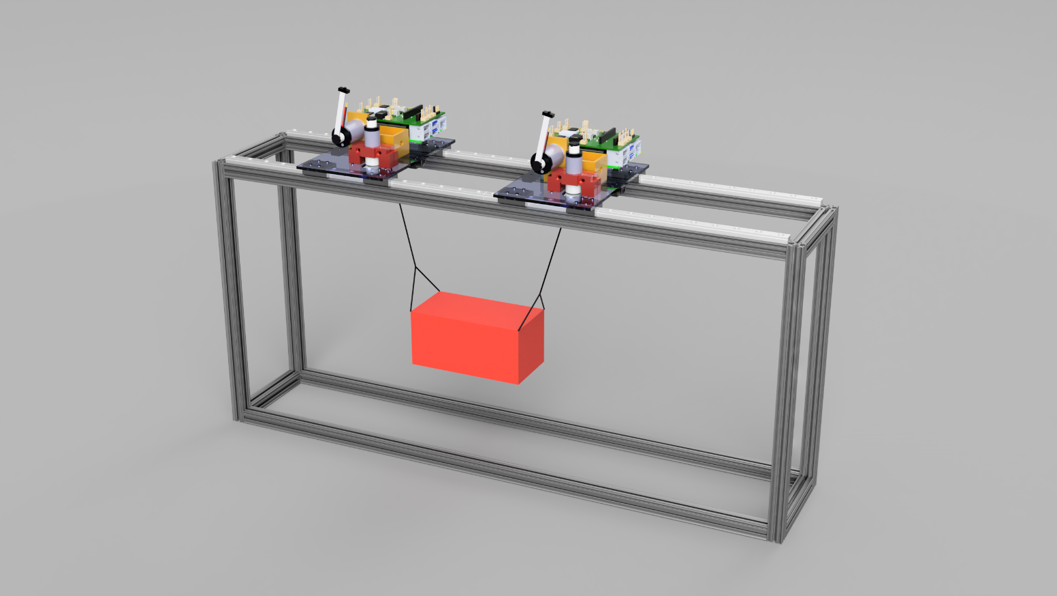
\includegraphics[width=110mm]{images/Veritas_demo_CAD}
	\end{center}

\end{frame}

%%%%%%%%%%%%%%%%%%%%%%%%%%%%%%%%%%%%%%%%%%%%%%%%%%%%%%%%%%%%

\begin{frame}<1>[label=sysbeschr2]
	\frametitle{System- {\color<1-3>{mygray} und Problembeschreibung}}
	\begin{center}
		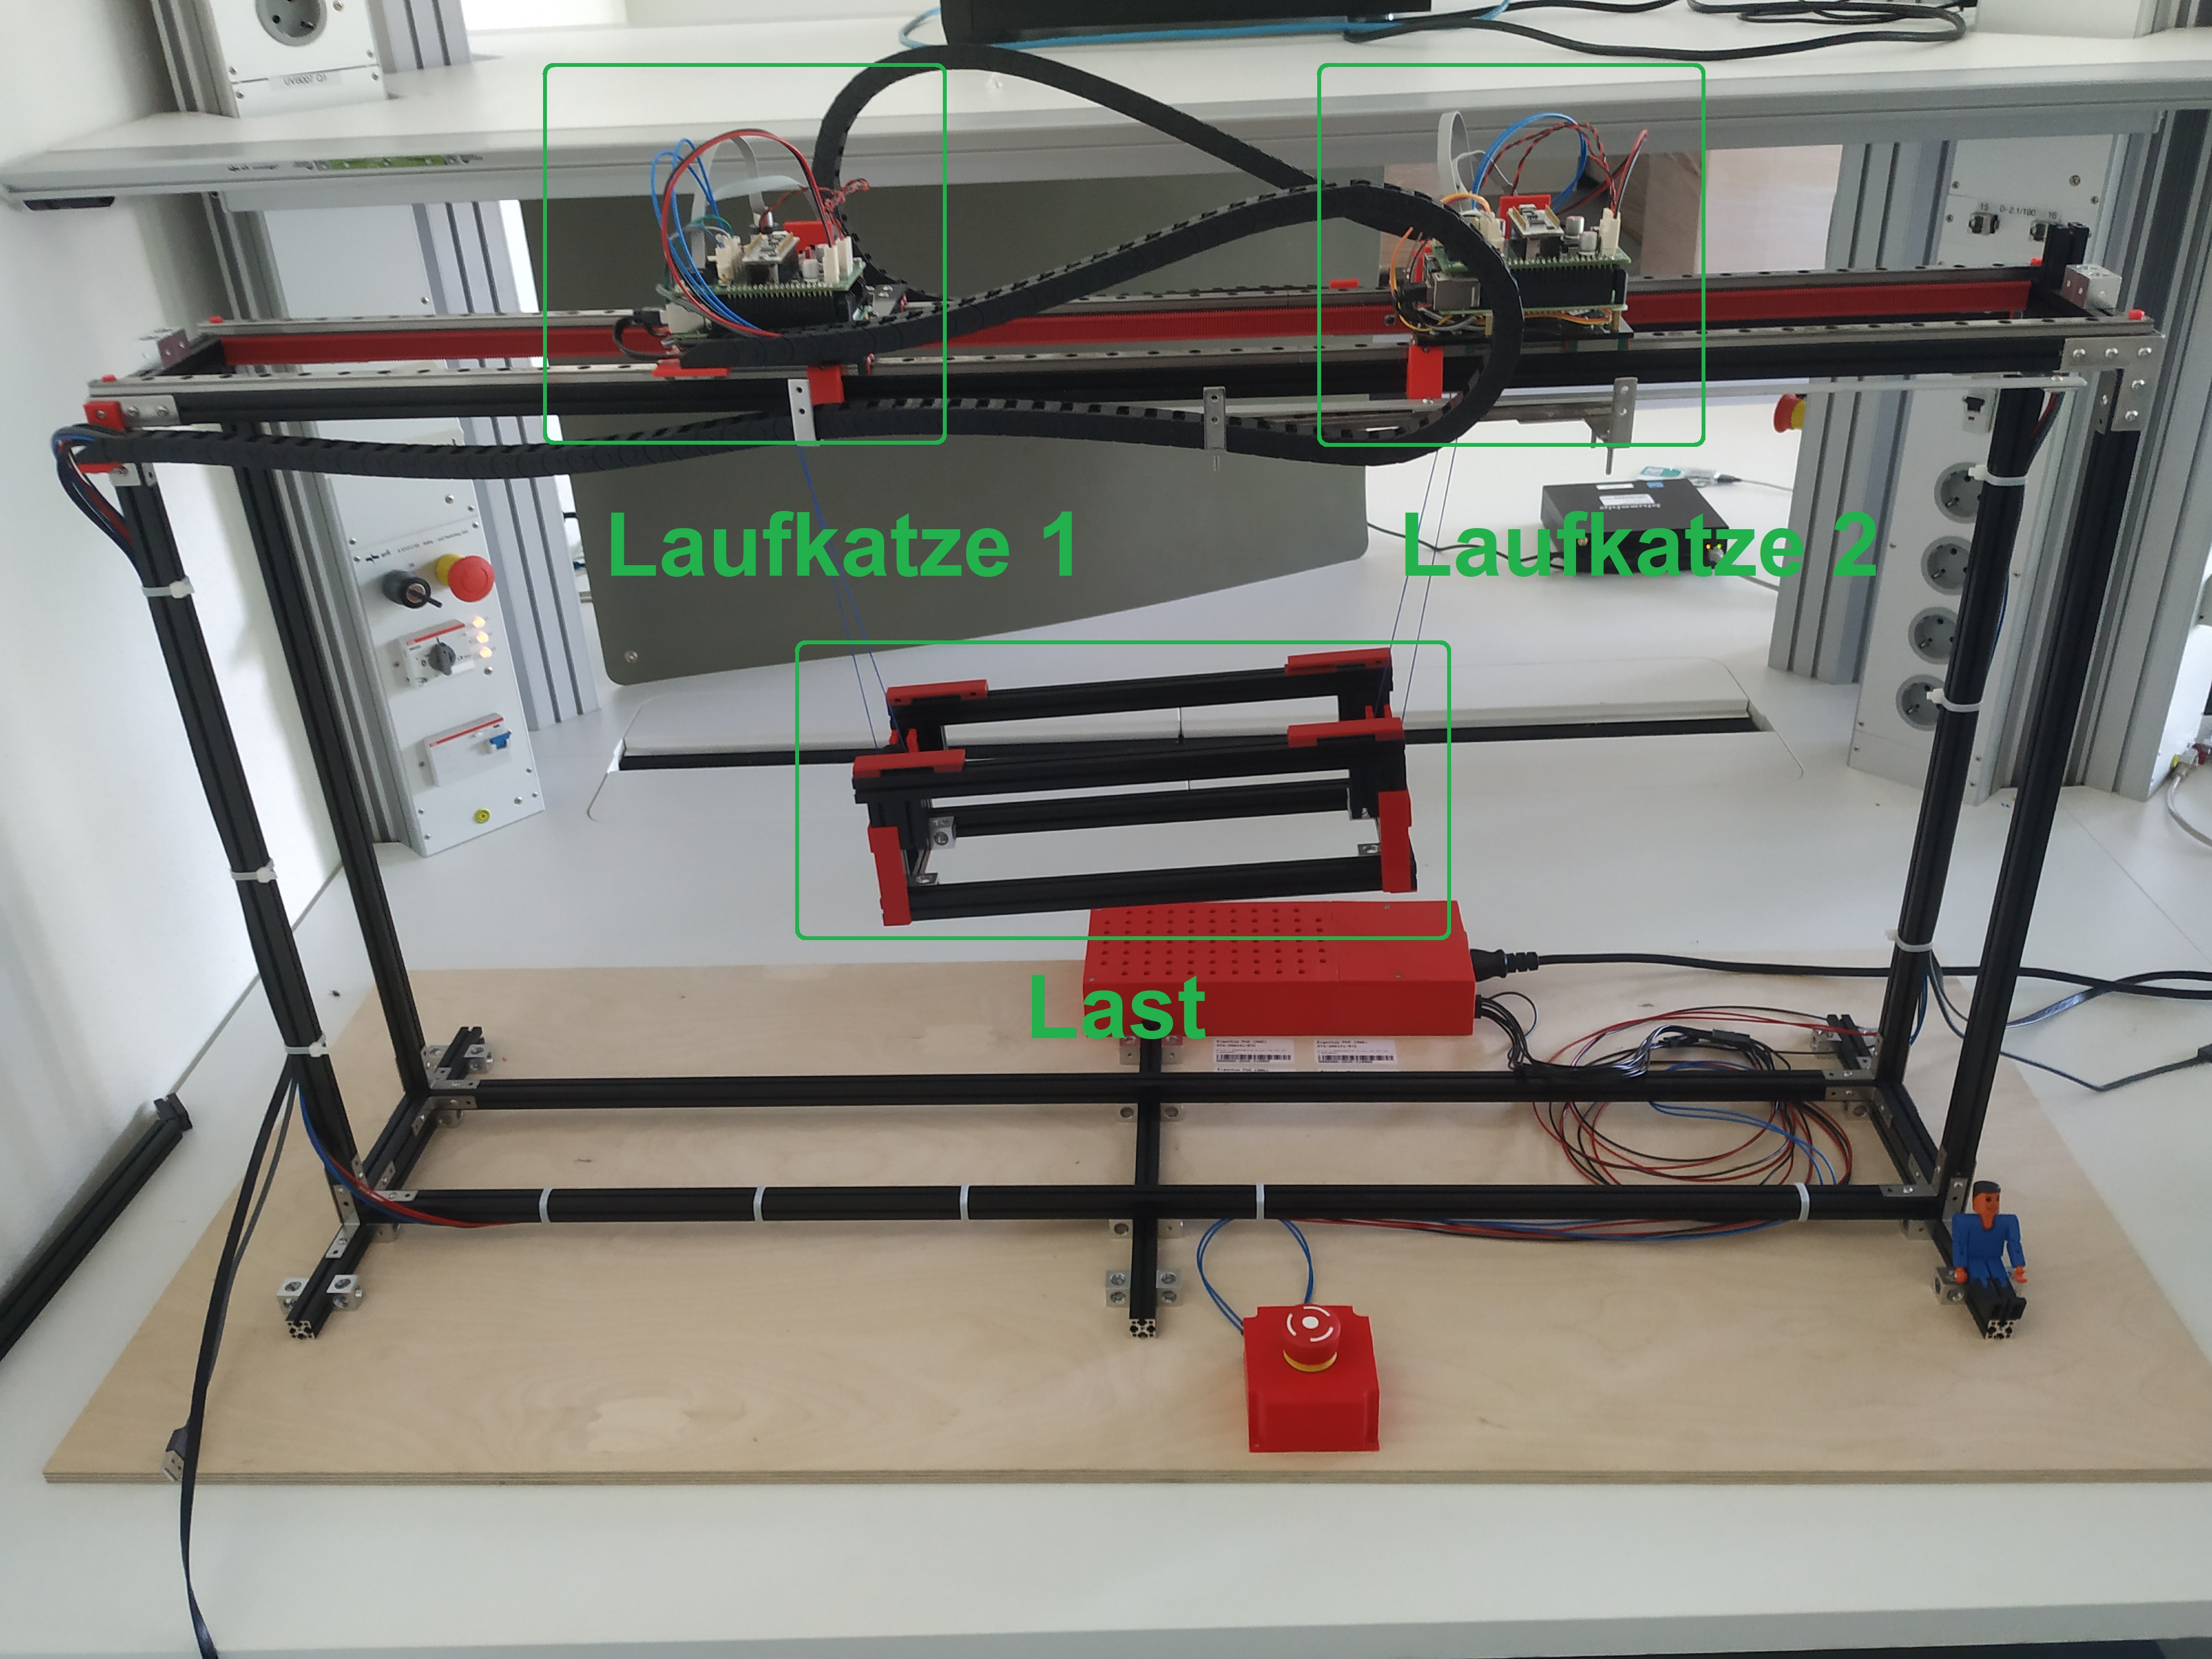
\includegraphics[width=85mm]{images/real_gantry}
	\end{center}
	
\end{frame}

%%%%%%%%%%%%%%%%%%%%%%%%%%%%%%%%%%%%%%%%%%%%%%%%%%%%%%%%%%%%

\begin{frame}[label=sysbeschr3]
	\frametitle{System- und Problembeschreibung}
	\textbf{Zielsetzung}
	\begin{itemize}
		\item Ruckarme Überführung der Last zwischen Ruhelagen in der vertikalen Aufhängungsebene
		\pause
		\item Zentrale Trajektorienplanung und Referenzregelstrategie unter Vorgabe von Sollposen der Last
		\pause
		\item Regelungsentwurf auf Basis von Modellierung des Versuchsstands als Mehrkörpersystem
		\pause  
		\item Perspektivisch Vergleich der zentralen Regelung mit verteilten Regelungsansätzen und Grundlage für maschinelles Lernen 
	\end{itemize}
\end{frame}

%%%%%%%%%%%%%%%%%%%%%%%%%%%%%%%%%%%%%%%%%%%%%%%%%%%%%%%%%%%%

\begin{frame}<1>[label=gl2]
	\frametitle{Gliederung}
	\begin{itemize}
		%0
		\item[\cdbox] System- und Problembeschreibung
		%1
		\item[\only<1>{$\rightarrow$}\only<2>{$\rightarrow$}\only<3->{\cdbox}]
		\textbf<1>{Analytische Modellbildung}
		%2
		\item[\only<1>{$\square$}\only<2>{$\rightarrow$}\only<3->{\cdbox}]
		\textbf<2>{Flachheitsanalyse}
		%3
		\item[\only<1-2>{$\square$}\only<3>{$\rightarrow$}\only<4->{\cdbox}]
		\textbf<3>{Steuerungs- und Regelungsentwurf}
	\end{itemize}
\end{frame}

%%%%%%%%%%%%%%%%%%%%%%%%%%%%%%%%%%%%%%%%%%%%%%%%%%%%%%%%%%%%

\begin{frame}[label=analMB]
	\frametitle{Analytische Modellbildung}
	\textbf{Allgemeine Modellannahmen}
	\begin{itemize}
		\item Bewegung des Systems auf vertikale Ebene beschränkt
		\pause
		\item Seile mit vernachlässigbarer Masse gegenüber Laufkatzen, Last
		\pause
		\item Last trotz Aussparungen mit homogener Masseverteilung modelliert
		\pause
		\item Vernachlässigung dissipativer Kräfte 
	\end{itemize}

	\pause
	\bigskip
	\textbf{Vorgehen bei der Modellierung}
	\begin{itemize}
		\item Modellierung Einzelkran mit Lagrange-Gleichungen zweiter Art (LG2)
		\pause
		\item Modellierung Doppelkran mit LG2
		\pause
		\item (Modellierung Doppelkran mit Lagrange-Gleichungen erster Art)
	\end{itemize}
\end{frame}

%%%%%%%%%%%%%%%%%%%%%%%%%%%%%%%%%%%%%%%%%%%%%%%%%%%%%%%%%%%%

\begin{frame}[t,fragile,label=Lagrange2_1]{\large Lagrange-Formalismus}
	
	\textbf{Symbole}
	\begin{itemize}
		\item Konfigurationskoordinaten $\boldsymbol{\theta} = (\mathbf{q}, \mathbf{p})^T$
		\pause
		\item direkt aktuierte Koordinaten $\mathbf{q}$, nicht direkt aktuierte Koordinaten $\mathbf{p}$
		\pause
		\item kinetische Energie $T(\boldsymbol{\theta}, \dot{\boldsymbol{\theta}})$, potentielle Energie $V(\boldsymbol{\theta})$
		\pause
		\item Lagrange-Funktion $\mathcal{L}(\boldsymbol{\theta}, \dot{\boldsymbol{\theta}}) = T(\boldsymbol{\theta}, \dot{\boldsymbol{\theta}}) - V(\boldsymbol{\theta})$
		\pause
		\item verallgemeinerte Kraft $\mathbf{Q} = \mathbf{f} - \mathbf{D}$
		\pause
		\item äußere Stellkraft $\mathbf{f}$, interne Reibungskraft $\mathbf{D}$
	\end{itemize}
	
	\pause
	\bigskip
	\textbf{Lagrange-Gleichungen zweiter Art}
	\begin{itemize}
		\pause
		\item  $\boldsymbol{\theta}$ sind unabhängig (ohne Zwangsbedingung verkoppelt)
		\pause
		\item Bewegungsgleichungen:
		\begin{equation*}
			\frac{\mathrm{d}}{\mathrm{d} t} \left(\frac{\partial \mathcal{L}}{\partial \dot{\theta}_i} \right) - \frac{\partial \mathcal{L}}{\partial \theta_i} = Q_i, \quad i = 1, \ldots, n
		\end{equation*}
		\pause
		\item Woher $Q_i$?
	\end{itemize}
	
\end{frame}

%%%%%%%%%%%%%%%%%%%%%%%%%%%%%%%%%%%%%%%%%%%%%%%%%%%%%%%%%%%%

\begin{frame}[t,fragile,label=Lagrange2_2]{\large Lagrange-Formalismus}
	
	\textbf{Symbole}
	\begin{itemize}
		\item Konfigurationskoordinaten $\boldsymbol{\theta} = (\mathbf{q}, \mathbf{p})^T$
		\item verallgemeinerte Kraft $\mathbf{Q} = \mathbf{f} - \mathbf{D}$
		\pause
		\item Richtungsvektor zu $k$-tem massebehaftetem Partikel $\mathbf{r}_k$, Stellkraft $\mathbf{F}_k$ entlang $\mathbf{r}_k$
		\pause
		\item virtuelle Arbeit $\delta W$, virtuelle Verschiebung von Partikel $\delta \mathbf{r}_k$ und Koordinate $\theta_{i}$
	\end{itemize}
	
	\pause
	\bigskip
	\textbf{Prinzip der virtuellen Arbeit zur Bestimmung der $Q_i$}
	\begin{itemize}
		\pause
		\item  $\delta W = \sum_{k=1}^l \mathbf{F}_k \cdot \frac{\partial \mathbf{r}_k}{\partial \theta_1} \delta \theta_1 +\ldots + \sum_{k=1}^l \mathbf{F}_k \cdot \frac{\partial \mathbf{r}_k}{\partial \theta_n} \delta \theta_n$
		\pause
		\item $\delta \mathbf{r}_{k} = \sum_{i = 1}^{n} \frac{\partial\mathbf{r}_{k}}{\partial\theta_i} \delta \theta_i$
		\pause
		\item $\delta W = \sum_{k=1}^{l}\delta \mathbf{r}_k^T \mathbf{F}_k = Q_1 \delta \theta_1 + \ldots + Q_n\delta \theta_n$
		\pause
		\item[$\rightarrow$] $Q_i = \sum_{k=1}^l \left(\frac {\partial \mathbf{r_k}} {\partial \theta_i} \right)^T \mathbf {F}_{k} = \frac{\partial\delta W}{\partial \delta \theta_i} ,\quad i=1,\ldots, n$
	\end{itemize}
	
\end{frame}

%%%%%%%%%%%%%%%%%%%%%%%%%%%%%%%%%%%%%%%%%%%%%%%%%%%%%%%%%%%%

\begin{frame}[t,fragile,label=ModellEinzelkran_1]{\large Analytisches Modell Einzelkran}
	\begin{textblock*}{80mm}[0.,0.](12mm,13mm)	
		\visible<1->{
			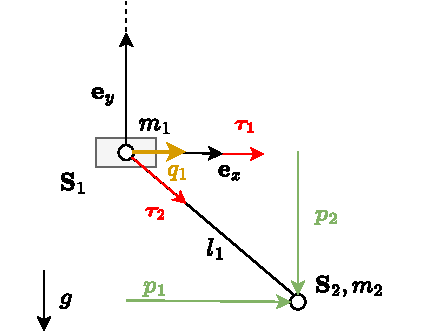
\includegraphics[width=64mm]{images/ODE_flatness_analysis_single_crane_diagram}
		}
		\bigskip
		\visible<2->{
			\begin{itemize}
				\item Massen bei $\mathbf{S}_1 = (q_1, 0)^T$, $\mathbf{S}_2 = (p_1, p_2)^T$
				\item variable Seillänge $l_1 = \sqrt{(p_1 - q_1)^2 + p_2^2}$\\
				~
			\end{itemize}
		}
	\end{textblock*}
	
	\begin{textblock*}{80mm}[0.,0.](80mm,13mm)
		
		\visible<3->{	
			\textbf{Energien:}			
			\begin{itemize}
				\item $T = \frac{m_1}{2} \dot{\mathbf{S}}_1^T \dot{\mathbf{S}}_1 + \frac{m_2}{2} \dot{\mathbf{S}}_2^T \dot{\mathbf{S}}_2 = \frac{m_{1} \dot{q}_{1}^{2}}{2} + \frac{m_{2} \dot{p}_{1}^{2}}{2} + \frac{m_{2} \dot{p}_{2}^{2}}{2}$
				\item $V = m_2 g \ \mathbf{S}_2^T \mathbf{e}_y = m_{2} g p_{2}$
			\end{itemize}
		}
		
	\end{textblock*}
	
	\begin{textblock*}{80mm}[0.,0.](80mm,35mm)
		
		\visible<4->{
			\textbf{Verallgemeinerte Kraft aus virtueller Arbeit:}
			\begin{itemize}
				\item $\mathbf{F}_1 =
				\left(\tau_{1}, 0 \right)^T$,
				$\mathbf{F}_2 =
				\left(\frac{\tau_{2} \left(p_{1} - q_{1}\right)}{l_{1}}, \frac{p_{2} \tau_{2}}{l_{1}} \right)^T$
				\item[$\rightarrow$] $\mathbf{Q} = \left(\frac{\tau_{2} \left(p_{1} - q_{1}\right)}{l_{1}}, \frac{p_{2} \tau_{2}}{l_{1}}, \tau_{1} - \frac{\tau_{2} \left(p_{1} - q_{1}\right)}{l_{1}} \right)^T$
			\end{itemize}
		}
		
	\end{textblock*}
	
\end{frame}

%%%%%%%%%%%%%%%%%%%%%%%%%%%%%%%%%%%%%%%%%%%%%%%%%%%%%%%%%%%%

\begin{frame}[t,fragile,label=ModellEinzelkran_2]{\large Analytisches Modell Einzelkran}
	\begin{textblock*}{80mm}[0.,0.](12mm,13mm)	
		\visible<1->{
			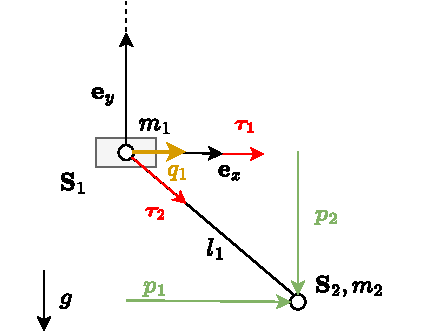
\includegraphics[width=64mm]{images/ODE_flatness_analysis_single_crane_diagram}
		}
		
		\visible<1->{
			\begin{itemize}
				\item Massen bei $\mathbf{S}_1 = (q_1, 0)^T$, $\mathbf{S}_2 = (p_1, p_2)^T$
				\item variable Seillänge $l_1 = \sqrt{(p_1 - q_1)^2 + p_2^2}$\\
				~
			\end{itemize}
		}
	\end{textblock*}
	
	\begin{textblock*}{80mm}[0.,0.](80mm,25mm)
		
		\visible<1->{
			\centering{\textbf{Systemgleichungen aus LG2:}}
			\begin{subequations}
				\label{single_flat_syseqs}
				\begin{flalign*}
					m_{2} \ddot{p}_{1} - \frac{\tau_{2} \left(p_{1} - q_{1}\right)}{l_{1}} &= 0\\
					g m_{2} + m_{2} \ddot{p}_{2} - \frac{p_{2} \tau_{2}}{l_{1}} &= 0\\
					m_{1} \ddot{q}_{1} - \tau_{1} + \frac{\tau_{2} \left(p_{1} - q_{1}\right)}{l_{1}} &= 0
				\end{flalign*}
			\end{subequations}
		}
		
	\end{textblock*}
	
\end{frame}

%%%%%%%%%%%%%%%%%%%%%%%%%%%%%%%%%%%%%%%%%%%%%%%%%%%%%%%%%%%%

\begin{frame}[t,fragile,label=ModellDoppelkran_1]{\large Analytisches Modell Doppelkran}
	\begin{textblock*}{80mm}[0.,0.](12mm,13mm)	
		\visible<1->{
			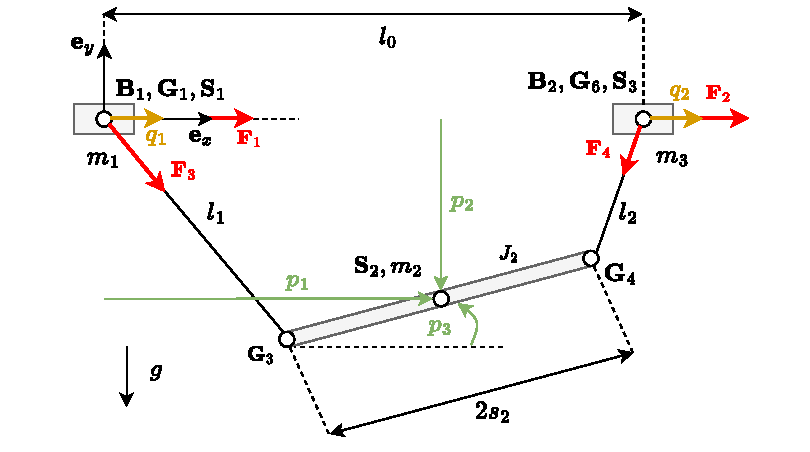
\includegraphics[width=64mm]{images/ODE_flatness_analysis_double_crane_diagram}
		}
		\bigskip
		\visible<2->{
		\textbf{variable Seillängen:}
		\tiny{
		\begin{flalign*}
			l_1 &= \sqrt{\left(p_{2} - s_{2} \sin{\left(p_{3} \right)}\right)^{2} + \left(p_{1} - q_{1} - s_{2} \cos{\left(p_{3} \right)}\right)^{2}}&& \\
			l_2 &= \sqrt{\left(p_{2} + s_{2} \sin{\left(p_{3} \right)}\right)^{2} + \left(- l_{0} + p_{1} - q_{2} + s_{2} \cos{\left(p_{3} \right)}\right)^{2}}&&
		\end{flalign*}
		}
		~
		}
	\end{textblock*}
	
	\begin{textblock*}{80mm}[0.,0.](80mm,13mm)
		
		\visible<3->{	
			\textbf{Energien:}			
			\begin{itemize}
				\item $T = \frac{J_{2} \dot{p}_{3}^{2}}{2} + \frac{m_{1} \dot{q}_{1}^{2}}{2} + \frac{m_{2} \dot{p}_{1}^{2}}{2} + \frac{m_{2} \dot{p}_{2}^{2}}{2} + \frac{m_{3} \dot{q}_{2}^{2}}{2}$
				\item $V =m_{2} g p_{2}$
			\end{itemize}
		}
	\end{textblock*}
	
	\begin{textblock*}{80mm}[0.,0.](80mm,35mm)
		
		\visible<4->{
			\textbf{Stellkräfte entlang Massepartikel:}
			\begin{flalign*}
				\mathbf{F}_1 &=
				\left( \tau_{1}, 0 \right)^T, \\
				\mathbf{F}_2 &=
				\left( \tau_{2}, 0 \right)^T, \\
				\mathbf{F}_3 &=
				\left(\begin{matrix}
					\frac{\tau_{3} \left(p_{1} - q_{1} - s_{2} \cos{\left(p_{3} \right)}\right)}{l_{1}}\\
					\frac{\tau_{3} \left(p_{2} - s_{2} \sin{\left(p_{3} \right)}\right)}{l_{1}}
				\end{matrix}\right), \\
				\mathbf{F}_4 &=
				\left(\begin{matrix}
					\frac{\tau_{4} \left(- l_{0} + p_{1} - q_{2} + s_{2} \cos{\left(p_{3} \right)}\right)}{l_{2}}\\
					\frac{\tau_{4} \left(p_{2} + s_{2} \sin{\left(p_{3} \right)}\right)}{l_{2}}
				\end{matrix}\right)
				\end{flalign*}
			}
		
	\end{textblock*}
	
\end{frame}

%%%%%%%%%%%%%%%%%%%%%%%%%%%%%%%%%%%%%%%%%%%%%%%%%%%%%%%%%%%%

\begin{frame}[t,fragile,label=ModellDoppelkran_2]{\large Analytisches Modell Doppelkran}
	\begin{textblock*}{80mm}[0.,0.](12mm,13mm)	
		\visible<1->{
			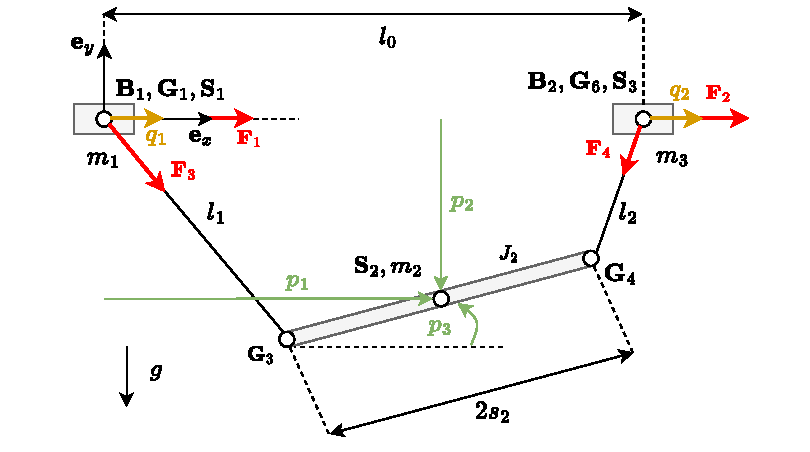
\includegraphics[width=64mm]{images/ODE_flatness_analysis_double_crane_diagram}
		}
		\bigskip
		\visible<1->{
			\textbf{variable Seillängen:}
			\tiny{
				\begin{flalign*}
					l_1 &= \sqrt{\left(p_{2} - s_{2} \sin{\left(p_{3} \right)}\right)^{2} + \left(p_{1} - q_{1} - s_{2} \cos{\left(p_{3} \right)}\right)^{2}}&& \\
					l_2 &= \sqrt{\left(p_{2} + s_{2} \sin{\left(p_{3} \right)}\right)^{2} + \left(- l_{0} + p_{1} - q_{2} + s_{2} \cos{\left(p_{3} \right)}\right)^{2}}&&
				\end{flalign*}
			}
			~
		}
	\end{textblock*}
	
	\begin{textblock*}{80mm}[0.,0.](80mm,13mm)
		
		\visible<1->{	
			\textbf{Verallgemeinerte Kraft aus virtueller Arbeit:}			
			\begin{equation*}
				\mathbf{Q}= ...
			\end{equation*}
		}
	\end{textblock*}

	\begin{textblock*}{80mm}[0.,0.](80mm,27mm)	
		\visible<2->{
			\textbf{Systemgleichungen aus LG2:}
			\tiny{
			\begin{flalign*}
			&m_{2} \ddot{p}_{1} - \frac{\tau_{4} \left(- l_{0} + p_{1} - q_{2} + s_{2} \cos{p_{3}}\right)}{l_{2}} - \frac{\tau_{3} \left(p_{1} - q_{1} - s_{2} \cos{p_{3}}\right)}{l_{1}} = 0\\
			&g m_{2} + m_{2} \ddot{p}_{2} - \frac{\tau_{4} \left(p_{2} + s_{2} \sin{p_{3}}\right)}{l_{2}} - \frac{\tau_{3} \left(p_{2} s_{2} \sin{p_{3}}\right)}{l_{1}} = 0\\
			&J_{2} \ddot{p}_{3} - \frac{s_{2} \tau_{4} \left(p_{2} + s_{2} \sin{p_{3}}\right) \cos{p_{3}} + s_{2} \tau_{4} \left(p_{1} - q_{2} + s_{2} \cos{p_{3}} - l_{0} \right)}{l_{2}}\\
			&+ \frac{s_{2} \tau_{3} \left(p_{2} - s_{2} \sin{p_{3}}\right) \cos{p_{3}}}{l_{1}} - \frac{s_{2} \tau_{3} \left(p_{1} - q_{1} - s_{2} \cos{p_{3}}\right) \sin{p_{3}}}{l_{1}} = 0\\
			&m_{1} \ddot{q}_{1} - \tau_{1} + \frac{\tau_{3} \left(p_{1} - q_{1} - s_{2} \cos{p_{3}}\right)}{l_{1}} = 0\\
			&m_{3} \ddot{q}_{2} - \tau_{2} + \frac{\tau_{4} \left(- l_{0} + p_{1} - q_{2} + s_{2} \cos{p_{3}}\right)}{l_{2}} = 0
			\end{flalign*}
			}
		}
		
	\end{textblock*}
	
\end{frame}

%%%%%%%%%%%%%%%%%%%%%%%%%%%%%%%%%%%%%%%%%%%%%%%%%%%%%%%%%%%%
\begin{frame}[t,fragile,label=ModellDoppelkran_3]{\large Analytisches Modell Doppelkran}
	\begin{textblock*}{80mm}[0.,0.](12mm,13mm)	
		\visible<1->{
			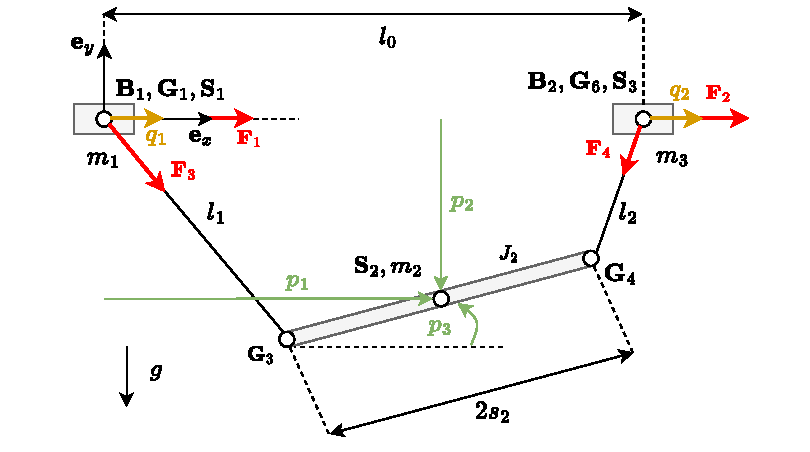
\includegraphics[width=64mm]{images/ODE_flatness_analysis_double_crane_diagram}
		}
		\bigskip
		\visible<1->{
			\textbf{variable Seillängen:}
			\tiny{
				\begin{flalign*}
					l_1 &= \sqrt{\left(p_{2} - s_{2} \sin{\left(p_{3} \right)}\right)^{2} + \left(p_{1} - q_{1} - s_{2} \cos{\left(p_{3} \right)}\right)^{2}}&& \\
					l_2 &= \sqrt{\left(p_{2} + s_{2} \sin{\left(p_{3} \right)}\right)^{2} + \left(- l_{0} + p_{1} - q_{2} + s_{2} \cos{\left(p_{3} \right)}\right)^{2}}&&
				\end{flalign*}
			}
			~
		}
	\end{textblock*}
	
	\begin{textblock*}{80mm}[0.,0.](80mm,13mm)
		
		\visible<1->{	
			\textbf{Eingangsaffines Zustandsraummodell:}			
		\begin{align}
			\label{eq:state_space_double_crane}
			\begin{split}
				\dot{\mathbf{x}} &= \mathbf{f}(\mathbf{x}) + \mathbf{g}(\mathbf{x}) \boldsymbol{\tau} \text{ mit } \\ 
				\mathbf{x} &= (p_{1},	p_{2}, p_{3}, q_{1}, q_{2}, \dot{p}_{1}, \dot{p}_{2}, \dot{p}_{3}, \dot{q}_{1}, \dot{q}_{2})^T, \\
				\mathbf{f}(\mathbf{x}) &= 
				(\dot{p}_{1}, \dot{p}_{2}, \dot{p}_{3}, \dot{q}_{1}, \dot{q}_{2}, 0, -g, 0, 0, 0)^T, \\ 
				\mathbf{g}(\mathbf{x}) &=
				\left(\begin{matrix}
					0 & 0 & 0 & 0\\
					0 & 0 & 0 & 0\\
					0 & 0 & 0 & 0\\
					0 & 0 & 0 & 0\\
					0 & 0 & 0 & 0\\
					0 & 0 & * & *\\
					0 & 0 & * & *\\
					0 & 0 & * & *\\
					* & 0 & * & 0\\
					0 & * & 0 & *
				\end{matrix}\right) \ \text{wobei} \ * \neq 0 
			\end{split}
		\end{align}
		}
	\end{textblock*}
	
\end{frame}

%%%%%%%%%%%%%%%%%%%%%%%%%%%%%%%%%%%%%%%%%%%%%%%%%%%%%%%%%%%%

\begin{frame}<1>[label=gl3]
	\frametitle{Gliederung}
	\begin{itemize}
		%0
		\item[\cdbox] System- und Problembeschreibung
		%1
		\item[\cdbox] Analytische Modellbildung
		%2
		\item[\only<1>{$\rightarrow$}\only<2>{$\rightarrow$}\only<3->{\cdbox}]
		\textbf<1>{Flachheitsanalyse}
		%3
		\item[\only<1-2>{$\square$}\only<3>{$\rightarrow$}\only<4->{\cdbox}]
		\textbf<2>{Steuerungs- und Regelungsentwurf}
	\end{itemize}
\end{frame}

%%%%%%%%%%%%%%%%%%%%%%%%%%%%%%%%%%%%%%%%%%%%%%%%%%%%%%%%%%%%

\begin{frame}[label=Flachheit_1]
	\frametitle{Flachheitsanalyse}
   	\begin{block}{Definition differenzieller Flachheit}
	Ein System der Form $\dot{\mathbf{x}} = \mathbf{F}(\mathbf{x}, \mathbf{u})$ mit $\mathbf{F}, \mathbf{x} \in \mathbb{R}^n$ und $\mathbf{u} \in \mathbb{R}^m$ heißt (differenziell) flach, falls ein $m$-Tupel $y := (y_1, ..., y_m)^T$ sowie glatte Funktionen $\mathbf{\Psi}$, $\boldsymbol{\theta}$ existieren, so dass
	\begin{align*}
			\mathbf{x} &= \mathbf{\Psi}(\mathbf{y}, \dot{\mathbf{y}}, ..., \mathbf{y}^{(n_x)}) \text{ mit } n_x < \infty \text{ und } \\
			\mathbf{u} &= \boldsymbol{\theta}(\mathbf{y}, \dot{\mathbf{y}}, ..., \mathbf{y}^{(n_u)}) \text{ mit } n_u < \infty \text{ gilt.}
	\end{align*}
	\end{block}

	\pause
	\bigskip
	\textbf{Erläuterungen:}
	\begin{itemize}
		\item Systemzustand $\mathbf{x}$, Systemeingang $\mathbf{u}$ 
		\item \textbf{flacher Ausgang} $\mathbf{y}$
		\item[$\rightarrow$] Parametrisierung aller Systemgrößen durch $\mathbf{y}$ und endlich viele Ableitungen ohne Lösung von DGL/Integration möglich
	\end{itemize}
\end{frame}

%%%%%%%%%%%%%%%%%%%%%%%%%%%%%%%%%%%%%%%%%%%%%%%%%%%%%%%%%%%%

\begin{frame}[t,fragile,label=Flachheit_2]{\large Flachheitsanalyse von MIMO-Systemen}
	
	\textbf{Prinzipielles Vorgehen}
	
	\begin{itemize}
		\pause
		\item  Eingangsaffines nichtlineares MIMO-System\\
		$\dot{\mathbf{x}} = \mathbf{f}(\mathbf{x}) + \mathbf{g}(\mathbf{x}) \mathbf{u}$ \quad mit \quad $\mathbf{x}, \mathbf{f} \in \mathbb{R}^n$, $\mathbf{u} \in \mathbb{R}^m$, $\mathbf{g} \in \mathbb{R}^{n \times m}$
		
		\pause
		\item Elimination von $\mathbf{u}$ durch jeweils eine Systemgleichungen
		\pause
		\item[$\rightarrow$] autonomes System aus $p := n - m$ Gleichungen
		\pause
		\item[$\rightarrow$] Elimination von $p$ Zustandskomponenten und aller übrigen Systemgleichungen
		\pause
		\item[$\rightarrow$] übrig bleiben $n - p = m $ Zustandskomponenten als \textbf{flacher Ausgang} $\mathbf{y}$
		\item Wie Systemgrößen und -gleichungen für Elimination auswählen?
	\end{itemize}
	
\end{frame}

%%%%%%%%%%%%%%%%%%%%%%%%%%%%%%%%%%%%%%%%%%%%%%%%%%%%%%%%%%%%

\begin{frame}[label=ef1]
  \frametitle{\large Motivation und Rückblick (1)}
  
  \textbf{Regelungstheorie hat heterogenes Methodenspektrum}
  \begin{itemize}
    \item PT1-Glied, ..., nichtlineare PDEs, ... \pause $\Rightarrow$ z.\,T. hochspezialisierte Mathematik
%    \item Lineare und nichtlineare Systemtheorie (Laplace, Ljapunov, ...)
%    \item[] Differentialgeometrie (Vektorfelder, ...), Funktionalanalysis (Funktionenräume, ...)
%    \item Theorie nichtlinearer dynamischer Systeme (Ljapunov-Theorie, periodische Orbits, ...) 
%    \item Differentialgeometrie (Vektorfelder, Lieableitungen, Differentialformen, Mannigfaltigkeiten, )
%    \item Funktionalanalysis (Funktionenräume, Skalarprodukte, Operatortheorie, ...)
%    \item Mathematisch geprägte Argumentation („Definition -- Satz -- Beweis“)

  \end{itemize}
  \pause
  \bigskip
  \textbf{Regelungstheorie hat heterogenes Anwendungsspektrum}
  \begin{itemize}
   \item Verfahrens-, Fahrzeug-, Gebäudetechnik, Robotik, ...
%     \item ...
%     \item $\Rightarrow$ Modelle und Problemstellungen aus vielen verschiedene Domänen
  \end{itemize}

  \bigskip
  \textbf{Beständiger Wissenszuwachs}
  \begin{itemize}
   \item überlineares Wachstum der Publikationen $\rightarrow$ Spezialisierung notwendig
  \end{itemize}

  \pause
  \bigskip
  \textbf{$\Rightarrow$ Wissenstransfer: nichttrivial}
  \begin{itemize}
   \item ... innerhalb der Regelungstechnik  
   \item ... in Anwendungsdomänen
  \end{itemize}

\end{frame}


%%%%%%%%%%%%%%%%%%%%%%%%%%%%%%%%%%%%%%%%%%%%%%%%%%%%%%%%%%%%%%%%%%%%%%%%%%%%%%%%

% 
% \begin{frame}[label=ef2]
%   \frametitle{\large Motivation und Rückblick (2)}
% \end{frame}



%%%%%%%%%%%%%%%%%%%%%%%%%%%%%%%%%%%%%%%%%%%%%%%%%%%%%%%%%%%%%%%%%%%%%%%%%%%%%%%%

% Tabelle 2021

%%%%%%%%%%%%%%%%%%%%%%%%%%%%%%%%%%%%%%%%%%%%%%%%%%%%%%%%%%%%%%%%%%%%%%%%%%%%%%%%


% 
% 
% \newlength{\vskp}
% \setlength{\vskp}{2mm}
% 
% \begin{frame}<4>[plain,label=rt1]
% % \begin{frame}[plain,label=rt1]
% \frametitle{\large Motivation und Rückblick (2): Regelungstheoretisches Wissen}
% 
% ~
% 
%   
%   \begin{columns}
% \column[t]{0.15\textwidth}
% 
% \textbf{Begriffe}\\[12mm]
% 
% \textbf{Zusammen\-hänge}\\[9mm]
% 
% 
% \textbf{Methoden}\\[12mm]
% 
% \textbf{Modelle}
% 
% \column[t]{0.30\textwidth} %%%%%%%%%%%%%%%%%%%%%%%%%%%%%%%%
% \visible<2->{
% ~\\[-1mm]
% Linearität, Steuerbarkeit, Flachheit, ...\\[7.5mm]
% 
% \textit{Jedes steuerbare lineare System ist flach.}\\[8mm]
% 
% <Transformation in Regelungsnormalform>\\[9mm]
% 
% $\dot {\mathbf{x}} = \mathbf{f}(\mathbf{x}, \mathbf{u})$\\
% ${\mathbf{y}} = \mathbf{h}(\mathbf{x})$\\
% }
% 
% \column[t]{0.03\textwidth} %%%%%%%%%%%%%%%%%%%%%%%%%%%%%%%%
% \visible<3->{
% ~\\[-1mm]
% $\rightarrow$\\[12mm]
% 
% $\rightarrow$\\[13mm]
% 
% $\rightarrow$\\[12mm]
% 
% $\rightarrow$
% }
% 
% 
% \column[t]{0.13\textwidth} %%%%%%%%%%%%%%%%%%%%%%%%%%%%%%%%
% \visible<3->{
% ~\\[-1mm]
% Definitionen\\[12mm]
% 
% 
% Sätze\\[13mm]
% 
% 
% Algorithmen\\[12mm]
% 
% Formeln
% }
% 
% \column[t]{0.03\textwidth} %%%%%%%%%%%%%%%%%%%%%%%%%%%%%%%%
% \visible<4->{
% ~\\[-1mm]
% $\rightarrow$\\[12mm]
% 
% $\rightarrow$\\[13mm]
% 
% $\rightarrow$\\[12mm]
% 
% $\rightarrow$
% } % visible spalte normal
% 
% % \visible<7->{
% % ~\\[-25.5mm]
% % ~$\searrow$
% % }
% 
% \column[t]{0.21\textwidth} %%%%%%%%%%%%%%%%%%%%%%%%%%%%%%%%
% \visible<4>{
% ~\\[-1mm]
% Ontologien\\
% (OWL, RDF)\\[8mm]
% 
% Semantische Regeln\\[8mm]
% 
% } %visible
% 
% 
% \only<4-5>{
% Software\\
% (ACKREP)\\[8mm]
% 
% CAS-Code\\
% (ACKREP)
% 
% }
% \only<6>{
% „Software“\\[11mm]
% 
% „Software“
% 
% }
% 
% \only<7->{
% \vspace{-11mm}
% }
% 
% \only<7>{
% \textcolor{myorange}{Methodennetz}\\[11mm]
% 
% \only<7->{\vspace{11mm}}
% 
% „Software“
% 
% }
% \only<8>{
% Methodennetz\\[8mm]
% 
% 
% \textcolor{myorange}{Automatic Control Knowledge Repository}
% 
% }
% 
% 
% \end{columns}
% 
% \begin{textblock*}{70mm}[0.,0.](90mm,14mm)
% \visible<3->{
% \textbf{„klassisch“:} \hspace{12mm}
% }
% \visible<4->{
% \textbf{„formal“:}
% }
% \end{textblock*}
% 
% 
% \begin{textblock*}{70mm}[0.,0.](130mm,25mm)
% \visible<5->{
% \only<5>{\textcolor{myorange}{OCSE}}
% \only<6->{OCSE}
% }
% % \rotatebox{10}{material}
% \end{textblock*}
% 
% 
% \end{frame}
% 
%%%%%%%%%%%%%%%%%%%%%%%%%%%%%%%%%%%%%%%%%%%%%%%%%%%%%%%%%%%%%%%%%%%%%%%%%%%%%%%%

\begin{frame}<1-2>[label=thesen]
  \frametitle{\large Thesen}
  
  
      \begin{block}{These 1}
        Die gegenwärtig dominierenden Medien (Fließtext, Formeln, Grafiken) der Wissensrepräsentation sind in Bezug auf die angesprochenen Probleme suboptimal.
    \end{block}
    
    \pause
    \bigskip
  
      \begin{block}{These 2}
        Formale Wissensrepräsentationsmethoden stellen eine vielversprechende Ergänzung dar.
    \end{block}
  
    \pause
    \bigskip
  
  % change color: https://tex.stackexchange.com/a/33235/2381
      \begin{block}{\textbf{These 3}}
        Bisher existierende technische Lösungen (OWL, Wikidata, ...) sind ungeeignet.
    \end{block}
    

\end{frame}


%%%%%%%%%%%%%%%%%%%%%%%%%%%%%%%%%%%%%%%%%%%%%%%%%%%%%%%%%%%%%%%%%%%%%%%%%%%%%%%%



\begin{frame}<1>[label=gl1]
  \frametitle{Gliederung}
  \begin{itemize}
   %0
   \item[\cdbox] Motivation und Rückblick
   %1
   \item[\only<1>{$\rightarrow$}\only<2->{\cdbox}]
     \textbf<1>{Formale Wissensrepräsentation: Ist-Stand}
   %2
   \item[\only<1>{$\square$}\only<2>{$\rightarrow$}\only<3->{\cdbox}]
     \textbf<2>{Ansatz: Emergent Representation of Knowledge (ERK)}
   %3
   \item[\only<1-2>{$\square$}\only<3>{$\rightarrow$}\only<4->{\cdbox}]
     \textbf<3>{Ontology of Control Systems Engineering (OCSE)}
   %4
   \item[\only<1-3>{$\square$}\only<4>{$\rightarrow$}\only<5->{\cdbox}]
     \textbf<4>{Zusammenfassung und Diskussion}
  \end{itemize}
\end{frame}


% ...

%%%%%%%%%%%%%%%%%%%%%%%%%%%%%%%%%%%%%%%%%%%%%%%%%%%%%%%%%%%%%%%%%%%%%%%%%%%%%%%%


%%%%%%%%%%%%%%%%%%%%%%%%%%%%%%%%%%%%%%%%%%%%%%%%%%%%%%%%%%%%%%%%%%%%%%%%%%%%%%%%

\begin{frame}[label=wr2]
  \frametitle{\large Formale Wissensrepräsentation (1): Begriffe}
  
\begin{columns}
\column[t]{1.02\textwidth}



\begin{block}{\textit{Eine} Ontologie [nach \textit{Studer et. al. 1998}]}
Maschinenverarbeitbare Spezifikation der begrifflichen Abdeckung einer Wissensdomäne.
\end{block}


\begin{itemize}
 \item[$\rightarrow$] Welche Begriffe gibt es? In welcher Beziehung stehen sie zueinander?
%  \item[] („Die Ontologie“ als Teildisziplin der Philosophie: „Lehre des Seins“ (Grundstruktur der Wirklichkeit) )
%  \item „Eine Ontologie“ (im Sinne der Informatik): Eine logische Theorie mit klar abgegrenztem Gültigkeitsbereich.
\end{itemize}

\pause

\begin{block}{Taxonomie}
Hierarchisches Klassifikationssystem von \texttt{ist-ein}-Beziehungen\\
\end{block}

\bigskip

 Beispiel: \texttt{Hauskatze} $\rightarrow$ \texttt{Säugetier} $\rightarrow$ \texttt{Wirbeltier} $\rightarrow$ \texttt{Lebewesen}

% \column[t]{0.18\textwidth}
\end{columns}  

%  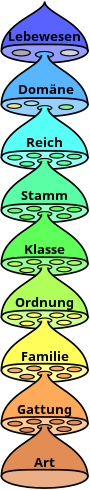
\includegraphics[width=1mm]{img/90px-Biological_classification_de.png}
%   \begin{textblock*}{40mm}[0.,0.](124mm,87mm)
% \visible<6->{
% {\tiny Quelle: \tcblue{\href{https://de.wikipedia.org/wiki/Taxonomie\#/media/Datei:Biological\_classification\_de.svg}{wikipedia.org/...}} (CC0)}
% }
% \end{textblock*}


\end{frame}

%%%%%%%%%%%%%%%%%%%%%%%%%%%%%%%%%%%%%%%%%%%%%%%%%%%%%%%%%%%%%%%%%%%%%%%%%%%%%%%%

\begin{frame}[label=wr3]
  \frametitle{\large Formale Wissensrepräsentation (2): Wissensgraphen {\color<1-2>{mygray}und RDF}}
  
\begin{textblock*}{80mm}[0.,0.](12mm,13mm)
 
\visible<1->{
  \textbf{„Knowledge Graph“:}
  \begin{itemize}
   \item Knoten: Begriffe
   \item Kanten: Beziehungen\\
   ~
  \end{itemize}
  
  
}
   
\visible<2->{
  
\includegraphics[width=64mm]{img/1280px-Semantic_Net}
}
\end{textblock*}
  
  
    \begin{textblock*}{40mm}[0.,0.](30mm,77mm)
\visible<2->{
{\tiny Quelle: \tcblue{\href{https://en.wikipedia.org/wiki/Semantic\_network\#/media/File:Semantic\_Net.svg}{wikipedia.org/...}} (CC0)}
}
\end{textblock*}
  

% \pause  
% \begin{itemize}
%     \item Eine Ontologie kann als Wissensgraph repräsentiert werden
% \end{itemize}


\begin{textblock*}{80mm}[0.,0.](80mm,13mm)
 
\visible<3->{
 
  \textbf{R}essource \textbf{D}escription \textbf{F}ramework:

 
  \begin{itemize}
%    \item Vom W3C als reines Metadaten-Modell konzipiert
   \item Sprache zur Beschreibung von Subjekt-Prädikat-Objekt-Tripeln
   \item[] \hspace{50mm} 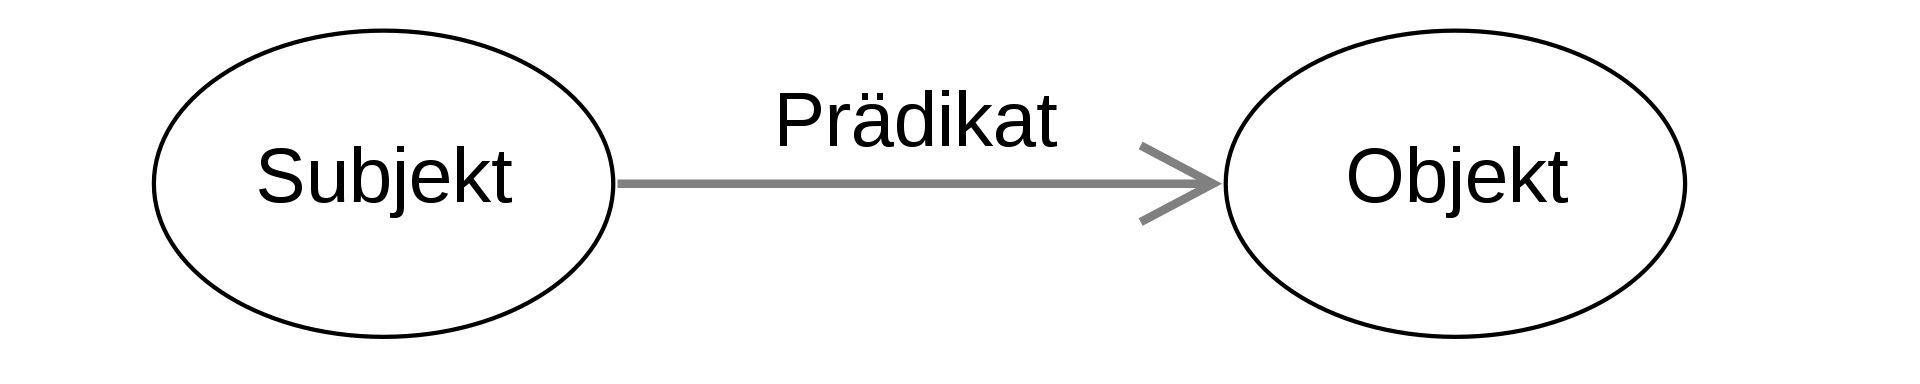
\includegraphics[width=50mm]{img/langde-1920px-Basic_RDF_Graph}
%    \item RDF\textbf{S}: Schema; beschreibt grundlegende Semantik (Subklassen, Subeigenschaften)
%    \item[$\Rightarrow$] Interpretation als „logische Theorie“ \\(Prädikatenlogik 1. Stufe)
%    
   \item[] 
%    \item Tripel-Elemente: Literale (\texttt{123}, \texttt{``xyz''}) oder (URIs \texttt{http://abc.de/pfad\#fragment})
%   \item<4-> Basissprache des \textit{„Semantic Web“} 
%    \item Maschinen-verabeitbare Dokumente
%    \item Überwindung sog. „Datensilos“ \\  (Bsp.: Getrennte Datebanken zu Genen und Proteinen)
   \item Zugehörige Abfragesprache:\\
   
   \smallskip
   \textbf{SPARQL} \\
   
   \smallskip
   (\underline{S}PARQL \underline{P}rotocol \underline{A}nd \underline{R}DF \underline{Q}uery \underline{L}anguage)

  \end{itemize}
  
  }

\end{textblock*}
% 

\end{frame}



%%%%%%%%%%%%%%%%%%%%%%%%%%%%%%%%%%%%%%%%%%%%%%%%%%%%%%%%%%%%%%%%%%%%%%%%%%%%%%%%

\begin{frame}[fragile,label=wr6]
  \frametitle{\large Formale Wissensrepräsentation (3): OWL {\color<1>{mygray}und Inferenz}}
  
  \textbf{W}eb \textbf{O}ntology \textbf{L}anguage
  \begin{itemize}
   \item OWL2: definierter Standard; basiert auf RDF
   \item Theoretische Basis: Beschreibungslogik(en)
   \begin{itemize}
    \item „Profile“ mit Unterschiedlicher Ausdrucksstärke %(z.\,B. transitive Eigenschaften, Kardinalitäten)
    \item Entscheidbare Fragmente der Prädikatenlogik 1. Stufe
    \item[$\Rightarrow$] Einfluss auf Komplexität von Inferenz-Algorithmen
%     \item Klassen („Konzepte“), Eigenschaften („Rollen“), Instanzen („Individuen“)
%     \item \href{https://en.wikipedia.org/wiki/Description_logic}{Beispiele}: $\mathcal{ALC}$, $\mathcal {SROIQ}^{\mathcal {(D)}}$
   \end{itemize}
% \item OWL-Klassenrestriktionen \texttt{owl:UnionOf}, \texttt{owl:minCardinality}, ...
% \texttt{owl:allValuesFrom},
% https://www.w3.org/TR/owl-test/byFunction#function-oneOf
  \end{itemize}

% \pause
% 
% \medskip
% 
% % \textbf{Beispiel}:
% \lstset{
%   basicstyle=\fontsize{10}{11}\selectfont\ttfamily
% }  
% \begin{lstlisting}
% @prefix demo: <http://demo.xy/onto#> .
% :pole rdf:type owl:Class.               # Klasse
% :has_pole rdf:type owl:ObjectProperty.  # Eigenschaft
% 
% :typical_transfer_func rdf:type owl:Class ;
%                 owl:equivalentClass [ rdf:type owl:Restriction ;
%                                 owl:onProperty :has_pole ;
%                                 owl:someValuesFrom :pole
%                                 ].      # Klassenrestriktion
% \end{lstlisting}


\medskip
\pause


  \textbf{Inferenzsystem} („Schließer“ bzw. Reasoner)
  \begin{itemize}
   \item Kann Schlussfolgerungen aus Behauptungen (Axiomen) ableiten
%    \begin{itemize}
%    \item[$\Rightarrow$] (Re)Klassifikation von Instanzen
%    \end{itemize}
   \smallskip
   \item Kann Inkonsistenzen aufdecken (widersprüchliche Axiome identifizieren)
   \item Kann implizit enthaltene Informationen explizit machen („Logikrätsel lösen“)
  \end{itemize}

  
\end{frame}



%%%%%%%%%%%%%%%%%%%%%%%%%%%%%%%%%%%%%%%%%%%%%%%%%%%%%%%%%%%%%%%%%%%%%%%%%%%%%%%%


%%%%%%%%%%%%%%%%%%%%%%%%%%%%%%%%%%%%%%%%%%%%%%%%%%%%%%%%%%%%%%%%%%%%%%%%%%%%%%%%
\begin{frame}<1-6>[label=wr7]
  \frametitle{\large Formale Wissensrepräsentation (4): Wikidata {\color<1-3>{mygray} und SPARQL}}

  
\only<1->{
\begin{itemize}
 \item Weltweit größter frei zugänglicher Wissensgraph
 \item Kollaborativ erstellt, von Wikimedia Foundation organisiert
 \item $\exists$ \textit{Item}s: u.\,a. zu jedem Wikipedia-Eintrag:
 
 \pause
 \begin{itemize}
  \item \url{https://www.wikidata.org/wiki/Q252446} \textit{Anif bei Salzburg}
  \item \texttt{https://www.wikidata.org/wiki/Q4917288} \textit{Control Engineering}
 \end{itemize}
 
 \pause
 \smallskip
 \item $\exists$ \textit{Properties}:
 \begin{itemize}
  \item \texttt{https://www.wikidata.org/wiki/P31} \textit{is instance of}
  \item \texttt{https://www.wikidata.org/wiki/P2534} \textit{has definig formula}
 \end{itemize}
 
 \item $\exists$ Statements (Kanten im Wissensgraph)

 \pause
 
 \smallskip
 \item Abfrageschnittstelle über SPARQL
 
 \pause
 \bigskip
 \item[$\rightarrow$] Repräsentation von mathematischen Inhalten in WD: umfangreich
 \item<6->[$\lightning$]  Repräsentation von regelungstheoretischen Inhalten in WD: \textbf{dürftig}
\end{itemize}

}
\pause

% https://query.wikidata.org/#SELECT%20%20%3Fitem%20%3FitemLabel%20%3Fformula%0AWHERE%20%0A%7B%0A%20%20%3Fitem%20wdt%3AP31%20wd%3AQ877802.%20%20%20%23%20P31%20%E2%86%92%20instance%20of%3B%20Q877802%20%E2%86%92%20integral%20transformation%0A%20%20%3Fitem%20wdt%3AP2534%20%3Fformula.%20%20%20%23%20P2534%20%E2%86%92%20definig%20formula%0A%20%20SERVICE%20wikibase%3Alabel%20%7B%20bd%3AserviceParam%20wikibase%3Alanguage%20%22%5BAUTO_LANGUAGE%5D%2Cen%22.%20%7D%0A%7D


\begin{textblock*}{\textwidth}[0.,0.](5mm,0mm)
\visible<5>{
 
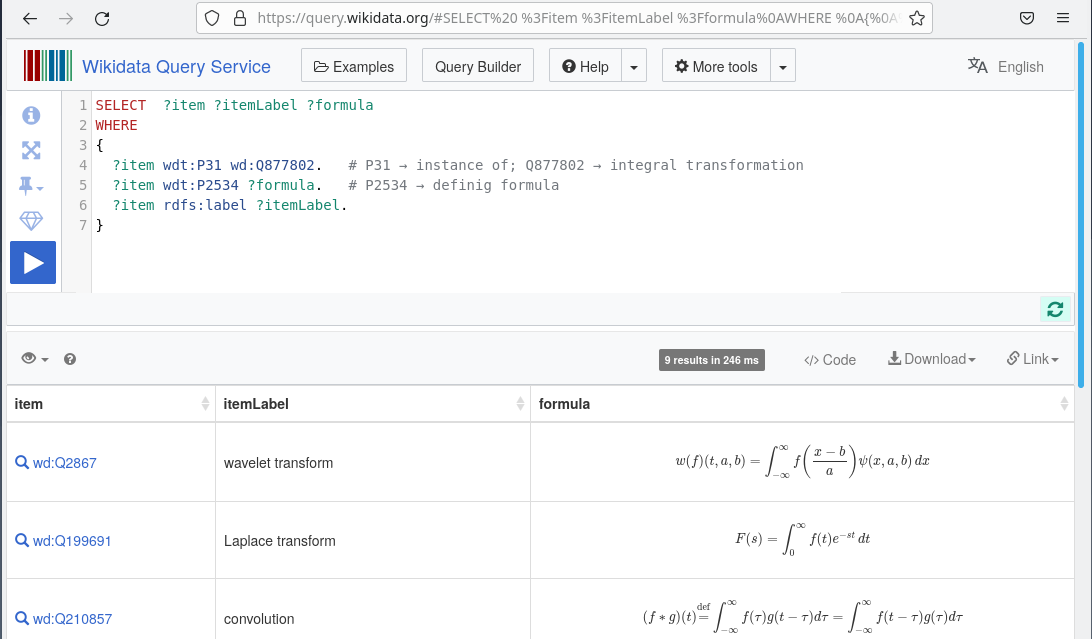
\includegraphics[width=1.1\textwidth,valign=t]{img/wd2}
}
\end{textblock*}

\begin{textblock*}{\textwidth}[0.,0.](5mm,0mm)
\visible<7>{
 
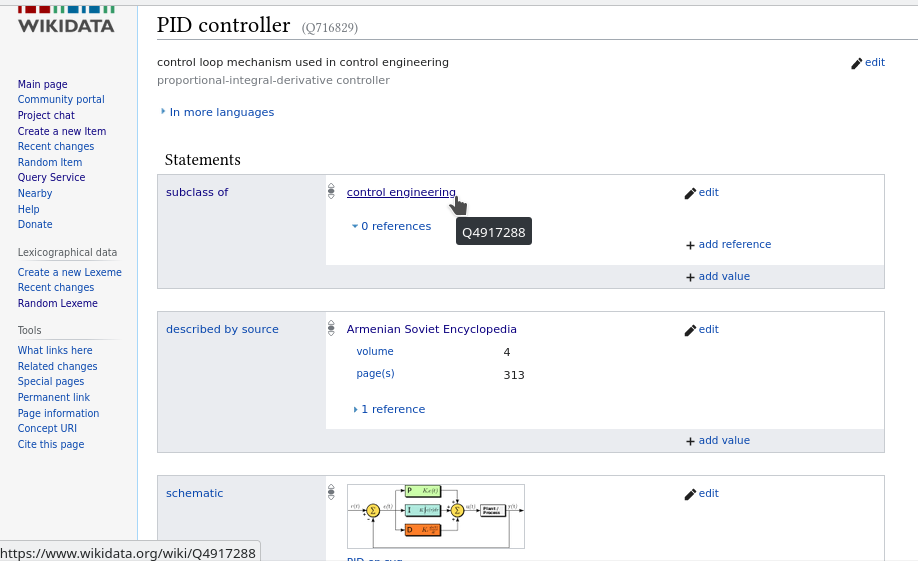
\includegraphics[width=1.1\textwidth,valign=t]{img/wd-pid-controller}
}
\end{textblock*}
  
\end{frame}



%%%%%%%%%%%%%%%%%%%%%%%%%%%%%%%%%%%%%%%%%%%%%%%%%%%%%%%%%%%%%%%%%%%%%%%%%%%%%%%%


%%%%%%%%%%%%%%%%%%%%%%%%%%%%%%%%%%%%%%%%%%%%%%%%%%%%%%%%%%%%%%%%%%%%%%%%%%%%%%%%
\againframe<3->{thesen}

%%%%%%%%%%%%%%%%%%%%%%%%%%%%%%%%%%%%%%%%%%%%%%%%%%%%%%%%%%%%%%%%%%%%%%%%%%%%%%%%
\againframe<2>{gl1}

%%%%%%%%%%%%%%%%%%%%%%%%%%%%%%%%%%%%%%%%%%%%%%%%%%%%%%%%%%%%%%%%%%%%%%%%%%%%%%%%


\begin{frame}[fragile,label=erk1]{\large Experimenteller Ansatz: ERK}


\textbf{Verklemmung:}

\smallskip

\circled{1} Kein {\color<3->{myblue} geeigneter} Repräsentationsformalismus  $\rightarrow$ \circled{2} Keine Inhalte $\rightarrow$ \circled{3} Keine Anwendungen 
$\rightarrow$ \circled{4} Keine Aufmerksamkeit $\rightarrow$ \circled{5} Keine Entwicklung $\rightarrow$ \circled{1}

\pause
\bigskip

\textbf{Pragmatischer Ansatz:}
\begin{itemize}
 \item[\circled{1}]  {Repräsentationsformalismus}: \textbf{E}mergent \textbf{R}epresentation of \textbf{K}nowledge
 \item[{\color<3->{mygray}  \circled{2}}] {\color<3->{mygray}  initiale Inhalte: OCSE}
\end{itemize}

\pause
\bigskip

\textbf{Anforderungen}
\begin{itemize}
\item Fokus auf Ausdrucksstärke \tikz[remember picture] \node[coordinate,xshift=16mm,yshift=1.0em] (n1) {};
\item Basiert auf menschenlesbarem Text 
\item Unterstützung für Automatisierung  \tikz[remember picture] \node[coordinate,yshift=-0.2em] (n2) {};
\end{itemize}

\visible<4->{

\begin{tikzpicture}[overlay,remember picture]
      \path (n2) -| node[coordinate] (n3) {} (n1);
      \draw[thick,decorate,decoration={brace,amplitude=3pt}]
            (n1) -- (n3) node[midway, right=4pt] {};
  \end{tikzpicture}
  
\begin{textblock*}{80mm}[0.,0.](80mm,63mm)
\visible<4->{
  Erfüllt von Allzweckprogrammiersprache\\ z.\,B. Python\\
}
\end{textblock*}
  

}


  
  
  \end{frame}
%%%%%%%%%%%%%%%%%%%%%%%%%%%%%%%%%%%%%%%%%%%%%%%%%%%%%%%%%%%%%%%%%%%%%%%%%%%%%%%%
  
\begin{frame}[t,fragile,label=erk2]{\large ERK: Imperative statt deklarative Wissensrepräsentation}

\textbf{Deklarativ}
\begin{itemize}
 \item Formuliert in \textit{Beschreibungs}sprache (z.B. OWL (Turtle Syntax))
\end{itemize}




% \begin{textblock*}{40mm}[0.,0.](12mm,27mm)
% \visible<2>{
% 
\includegraphics{img/listing2}
% }
% \end{textblock*}

\lstset{
  basicstyle=\fontsize{8}{11}\selectfont\ttfamily
}  
\begin{lrbox}{\mysaveboxa}
\begin{lstlisting}
I3749 rdfs:label "Cayley-Hamilton theorem".
I3749 rdfs:comment "every square matrix is a root of its own char. poly.".
I3749 rdf:type :I15_implication_proposition.
\end{lstlisting}
\end{lrbox}


\only<2->{
\medskip
\usebox{\mysaveboxa}
}

% https://tex.stackexchange.com/questions/250052/custom-lstlisting-highlighting-for-symbols
% %   basicstyle=\fontsize{8}{11}\selectfont\ttfamily,
% \lstset{
%   language=Python,
% %     showstringspaces=false,
%     backgroundcolor=\color{black!20},
% %     basicstyle=\lstfont{white},
% %     identifierstyle=\lstfont{white},
%     keywordstyle=\lstfont{magenta!40},
%     numberstyle=\lstfont{white},
% %     stringstyle=\lstfont{cyan},
% %     commentstyle=\lstfont{yellow!30},
%     emph={
%         cudaMalloc, label, I3749
%         __global__, __shared__, __device__, __host__,
%         __syncthreads,
%     },
%     emphstyle={\lstfont{green!60!white}},
%     breaklines=true
% }  

\begin{lrbox}{\mysaveboxb}
\begin{lstlisting}
I3749 = p.create_item(
    R1__has_label="Cayley-Hamilton theorem",
    R2__has_description="every square matrix is a root of its own char. poly.",
    R4__is_instance_of=p.I15["implication proposition"],
)
\end{lstlisting}
\end{lrbox}

\pause
\pause
\bigskip

\textbf{Imperativ}
\begin{itemize}
 \item Formuliert in \textit{Programmier}sprache (z.B. Python)
\end{itemize}
\visible<3>{
\usebox{\mysaveboxb}
}

\end{frame}
%%%%%%%%%%%%%%%%%%%%%%%%%%%%%%%%%%%%%%%%%%%%%%%%%%%%%%%%%%%%%%%%%%%%%%%%%%%%%%%%
  
\begin{frame}[t,fragile,label=erk3]{\large ERK: Imperative statt deklarative Wissensrepräsentation (2)}

\vspace{-2mm}

\textbf{Vorteile}
\begin{itemize}
 \item Direkte Programm-interne Repräsentation (kein Parsen)
 \item Direkte Erweiterbarkeit (Plugins im Graphen)
\end{itemize}

\pause
\bigskip
\textbf{Anwendung:} Geltungsbereiche (\textit{scopes})
\begin{itemize}
 \item Gliederung einer Aussage in \textit{Kontext-Etablierung}, \textit{Prämisse}, \textit{Behauptung}
 \item Gesamtaussage abhängig davon in welchem \textit{scope} eine Teilausage steht
 \item Deklarativ: nur sehr aufwendig umsetzbar
 \item Imperativ: einfach umsetzbar (automatisches Erzeugen von Hilfsknoten/kanten) 
\end{itemize}

\pause

\lstset{
  basicstyle=\fontsize{8}{11}\selectfont\ttfamily
}
\begin{lstlisting}
I3749 = p.create_item(
    R1__has_label="Cayley-Hamilton theorem",
    R2__has_description="every square matrix is a root of its own char. poly.",
    R4__is_instance_of=p.I15["implication proposition"],
)
\end{lstlisting}



% \textbf{Bemerkung:} Deklarativ funktioniert auch; Imperativ besser für Prototypenphase


\end{frame}
%%%%%%%%%%%%%%%%%%%%%%%%%%%%%%%%%%%%%%%%%%%%%%%%%%%%%%%%%%%%%%%%%%%%%%%%%%%%%%%%
  
\begin{frame}[t,fragile,label=erk5]{\large ERK - Beispiel: \textit{Inhalt} des Satzes von Cayley-Hamilton}

\vspace{-4mm}

\lstset{
  basicstyle=\fontsize{8}{11}\selectfont\ttfamily
}
\begin{lstlisting}
with I3749["Cayley-Hamilton theorem"].scope("context") as cm:
    cm.new_var(A=uq_instance_of(I9906["square matrix"]))
    cm.new_var(n=uq_instance_of(p.I39["positive integer"]))
\end{lstlisting}
\pause
\begin{lstlisting}
    cm.new_var(P=p.instance_of(I4240["matrix polynomial"]))
    cm.new_var(Z=p.instance_of(I9905["zero matrix"]))
\end{lstlisting}
\pause
\begin{lstlisting}
    cm.new_rel(cm.A, R5938["has row number"], cm.n)
    cm.new_rel(cm.A, R5940["has characteristic polynomial"], cm.P)
    cm.new_rel(cm.Z, R5938["has row number"], cm.n)
    cm.new_rel(cm.Z, R5939["has column number"], cm.n)
\end{lstlisting}
%     cm.new_rel(cm.Z, p.R24["has LaTeX string"], r"\mathbf{0}")
\pause
\begin{lstlisting}
with I3749["Cayley-Hamilton theorem"].scope("assertions") as cm:
    cm.new_equation(lhs=cm.P(cm.A), rhs=cm.Z)
\end{lstlisting}


\begin{textblock*}{50mm}[0.,0.](100mm,67mm)
\visible<4->{


\begin{tcolorbox}[colback=lightblue,colframe=softblue]

$P(\mathbf{A}) = \mathbf{Z}$ \quad mit $\mathbf{Z}:= \mathbf{0}$
\end{tcolorbox}
}
\end{textblock*}

\end{frame}

% \againframe<5>[plain]{erk5}
%%%%%%%%%%%%%%%%%%%%%%%%%%%%%%%%%%%%%%%%%%%%%%%%%%%%%%%%%%%%%%%%%%%%%%%%%%%%%%%%
  
\begin{frame}[t,fragile,label=erk4]{\large ERK-Inferenzsystem}

\textbf{Nachteile Imperativer Repräsentation}
\begin{itemize}
 \item ...
%  \item Unklare Interoperabilität („Insellösung“)
 \item Kein Einsatz existierender \textit{Reasoner}
\end{itemize}

\pause

\bigskip
\textbf{$\rightarrow$ Regelbasierte Inferenz}
\begin{itemize}
 \item Beispiel: Klassifikation von $\dot x = a\sin(x) + bx^2 + c x + u$
 \item \textit{Eingangsaffinität} $\supset$ \textit{Polynomialität} (a=0) $\supset$ \textit{Linearität} (a,b=0)  
\pause
 \item Im Graph: ~ \py|I4761["linear"]| ~ \py|R17["is subproperty of"]| ~ \py|I5247["polynomial"]|
 \item Wunsch: Schlussfolgerung von ~ \py|I4761["linear"]| ~ \py|R17| ~ \py|I6091["control affine"]|
\pause
 \item Abstrakt: Transitivität der Relation \py|R17["is subproperty of"]|
 \smallskip
 \item Wunsch: Regel soll selbst Teil des Wissensgraphen sein
 
\end{itemize}

\end{frame}
%%%%%%%%%%%%%%%%%%%%%%%%%%%%%%%%%%%%%%%%%%%%%%%%%%%%%%%%%%%%%%%%%%%%%%%%%%%%%%%%
  
\begin{frame}[t,fragile,label=erk6]{\large ERK-Inferenzsystem: Regelspezifikation}

\lstset{
  basicstyle=\fontsize{8}{11}\selectfont\ttfamily
}
\begin{lstlisting}
I400 = p.create_item(
    R1__has_label="transitivity of R17__is_subproperty_of",
    R4__is_instance_of=p.I41["semantic rule"],
)
\end{lstlisting}
\pause
\begin{lstlisting}
with I400["subproperty rule 1"].scope("context") as cm:
    cm.new_var(P1=p.instance_of(p.I11["mathematical property"]))
    cm.new_var(P2=p.instance_of(p.I11["mathematical property"]))
    cm.new_var(P3=p.instance_of(p.I11["mathematical property"]))
\end{lstlisting}
\pause
\begin{lstlisting}
with I400.scope("premises") as cm:
    cm.new_rel(cm.P2, p.R17["is subproperty of"], cm.P1)
    cm.new_rel(cm.P3, p.R17["is subproperty of"], cm.P2)
\end{lstlisting}
\pause
\begin{lstlisting}
with I400.scope("assertions") as cm:
    cm.new_rel(cm.P3, p.R17["is subproperty of"], cm.P1)
\end{lstlisting}
% \pause

\end{frame}
%%%%%%%%%%%%%%%%%%%%%%%%%%%%%%%%%%%%%%%%%%%%%%%%%%%%%%%%%%%%%%%%%%%%%%%%%%%%%%%%
  
\begin{frame}[fragile,label=erk7]{\large ERK-Inferenzsystem: Regelauswertung}

\begin{itemize}
 \item Für jede Regel: „Prototypgraphen“ konstruieren
 \begin{itemize}
  \item lokale Variablen aus \py{scope("context")} $\rightarrow$ Knoten
  \item Relationen aus \py{scope("premises")} $\rightarrow$ Kanten
 \end{itemize}
 
 \pause
 \bigskip
 \item Passende Knoten aus dem Gesamtgraph suchen
 \begin{itemize}
  \item Mathematisches Problem: \textbf{\textit{Subgraphisomorphismen}} finden
%   (Bijektive Abbildungen zwischen den Knoten, welche die (spezifizierte) Verzweigungsstruktur erhalten)
  \item $\exists$ VF2-Algorithmus (fertig implementiert)
 \end{itemize}
 
 \pause
 \bigskip
 \item Beziehungen aus \py|scope("assertions")| abstrahieren und anwenden


\end{itemize}



\end{frame}
%%%%%%%%%%%%%%%%%%%%%%%%%%%%%%%%%%%%%%%%%%%%%%%%%%%%%%%%%%%%%%%%%%%%%%%%%%%%%%%%
  

\begin{frame}[t,fragile,label=erk8]{\large ERK -- Bemerkungen }


\begin{itemize}
 
\setbeamercolor{normal text}{fg=mygray}
\usebeamercolor[fg]{normal text}

 \item[\tca{\textbullet}] Alle \textit{Item}s und \texttt{Relation}s haben eindeutige URI (z.\,B. \texttt{erk:/builtins\#I41})
 \item[\tca{\textbullet}] Unterstützung für Mehrsprachigkeit (Label, Beschreibung, ...)
 
 \item[\tca{\textbullet}] Unterstützung für Qualifier (Kanten, die auf Kanten zeigen)
 \begin{itemize}
  \item[\tca{\textbullet}] Semantische Information steckt in Knoten und Kanten
  \item[\tca{\textbullet}] menschenlesbare Texte sind Hilfsattribute
 \item[\tca{\textbullet}] Lesbarkeit für Mensch und Maschine:\quad \texttt{I41["{}semantische Regel"@de]} $\hat{=}$ \texttt{I41}
 \end{itemize}
 
%  \pause
 \medskip
 \item[\tca{\textbullet}] Zur Begriffswahl „Emergent“ (\underline{E}RK)
 

\begin{itemize}
 \item[\tca{\textbullet}] \textit{Emergenz} wörtlich: „das Auftauchen“
 \item[\tca{\textbullet}] Bedeutung: Phänomen, dass in komplexen Systemen Eigenschaften auftreten, die nicht aus den Eigenschaften der Elemte vorhergesagt werden können.
 \item[\tca{$\rightarrow$}]: \textit{Das Ganze ist mehr als die Summe seiner Teile.}
 
 \medskip
 \item[\tca{\textbullet}] Ursprünglich: ERK -- „\textit{Easy} Knowledge Representation“
\end{itemize}

\end{itemize}

 
\setbeamercolor{normal text}{fg=tublue}
\usebeamercolor[fg]{normal text}

\begin{itemize}
\item \textbf{$\exists$ RDF-Export $\rightarrow$ SPARQL Suche möglich}

\end{itemize}




\end{frame}
%%%%%%%%%%%%%%%%%%%%%%%%%%%%%%%%%%%%%%%%%%%%%%%%%%%%%%%%%%%%%%%%%%%%%%%%%%%%%%%%


\againframe<3>{gl1}

%%%%%%%%%%%%%%%%%%%%%%%%%%%%%%%%%%%%%%%%%%%%%%%%%%%%%%%%%%%%%%%%%%%%%%%%%%%%%%%%
% \againframe<2>[plain]{erk1}
  
\begin{frame}[fragile,label=ocse1]{\large \underline{O}ntology of \underline{C}ontrol \underline{S}ystems \underline{E}ngineering}

\textbf{2021: OCSE 0.1}
\begin{itemize}
 \item in OWL implementiert
 \item Taxonomie einfach umsetzbar
 \item Weitere Beziehungen schwierig  (mangelnde OWL-Ausdrucksstärke)
\end{itemize}

\pause
\bigskip
\textbf{2022: OCSE 0.2}
\begin{itemize}
 \item Basierend auf ERK implementiert
 \item Größere Modellierungstiefe möglich
\end{itemize}


\begin{textblock*}{40mm}[0.,0.](10mm,46mm)
\only<1>{

\includegraphics[width=140mm]{img/ocse-prototype01.pdf}
}
\end{textblock*}
% \begin{textblock*}{40mm}[0.,0.](75mm,13mm)
% \only<2>{
% %\includegraphics[trim=left bottom right top, clip]{file}
% 
\includegraphics[trim=300mm 0 1200mm 90mm, clip,width=80mm]{img/ocse-prototype01.pdf}
% }
% \end{textblock*}

\end{frame}
%%%%%%%%%%%%%%%%%%%%%%%%%%%%%%%%%%%%%%%%%%%%%%%%%%%%%%%%%%%%%%%%%%%%%%%%%%%%%%%%
  
\begin{frame}[t,fragile,label=ocse2]{\large OCSE -- Wie anfangen?}


\lstset{
  basicstyle=\fontsize{8}{11}\selectfont\ttfamily
}  
% \begin{itemize}
%  \item[]
% \end{itemize}
\vspace{-3mm}
 Worum geht es in der Regelungstheorie? $\rightarrow$ \pause Dynamische Systeme.
\pause
\begin{lstlisting}
I5948 = p.create_item(
    R1__has_label="dynamical system",
    R4__is_instance_of=p.I2["Metaclass"] # <- Metaklassen-Instanzen sind Klassen
)
\end{lstlisting}
% Was \textit{ist} ein System? \pause $\rightarrow$ Erstmal egal.

\smallskip
Geht es wirklich um Systeme? \pause $\rightarrow$ Es geht um \textit{Modelle}.
\pause
 

\vspace{-1em}
\begin{lstlisting}
I7641 = p.create_item(
    R1__has_label="general system model",
    R4__is_instance_of=p.I2["Metaclass"],
)
\end{lstlisting}

\vspace{-2em}
\pause
\begin{lstlisting}
R7641 = p.create_relation(
    R1__has_label="has approximation",
    R8__has_domain_of_argument_1=I5948["dynamical system"],
    R11__has_range_of_result=I7641["general system model"],
)
\end{lstlisting}


\end{frame}
%%%%%%%%%%%%%%%%%%%%%%%%%%%%%%%%%%%%%%%%%%%%%%%%%%%%%%%%%%%%%%%%%%%%%%%%%%%%%%%%
  
\begin{frame}[t,fragile,label=ocse3]{\large OCSE -- Repräsentation von Mathematik}

\begin{itemize}
 \item Regelungstheoretische Aussagen benötigen unverzichtbar Mathematik
%  \item Relevante mathematische Konzepte „von Grund auf“ einführen?
%  \hfill $\rightarrow$ unpraktikabel
%  
 \pause
 \medskip
 \item Pragmatischer Ansatz: Irgendwo anfangen und schrittweise ergänzen
\end{itemize}


 \pause
 \medskip

\textbf{Beispiel: \py{R8133["relative degree"]}} \\
% Subklasse von I5356["general system property"]
($\hat{=}$ $\frac{d}{dt}$-Ordnung des Systemausgangs, die erstmals explizit vom Eingang abhängt)

\pause
\smallskip
benötigt:

\smallskip
\begin{itemize}
 \item \py|I1371["iterated Lie derivative of scalar field"]|
 \pause
    \begin{itemize}
    \item[\textbullet] \py|I1347["Lie derivative of scalar field"]|
    \pause
        \begin{itemize}
        \item[\textbullet] \py|I2075["substitution"]|
        \item[\textbullet] \py|I3513["derivative w.r.t. scalar parameter"]|
        \item[\textbullet] \py|I2753["flow of a vector field"]|
        \item[\textbullet] \py|I9273["explicit first order ODE system"]|
        \end{itemize}
    \end{itemize}
\end{itemize}

$\ldots$


\begin{textblock*}{46mm}[0.,0.](110mm,47mm)
\visible<5->{


\begin{tcolorbox}[colback=lightblue,colframe=softblue,title=Lie Ableitung]
$\dot x = f(x) + g(x)u$\\
$y = h(x)$

\vspace{3mm}

$L_f h := \Big(\frac{d}{dt} \varphi_t^f (x)\Big)\Big|_{t=0}$
\end{tcolorbox}
}
\end{textblock*}


\end{frame}
%%%%%%%%%%%%%%%%%%%%%%%%%%%%%%%%%%%%%%%%%%%%%%%%%%%%%%%%%%%%%%%%%%%%%%%%%%%%%%%%
  
\begin{frame}[t,fragile,label=ocse4]{\large OCSE -- Status {\color<1-3>{mygray} und Anwendungen}}

\textbf{Status}: \texttt{<erk:/builtins>} $\cup$ \texttt{<erk:/ocse/0.2>}: $\approx$ 230 Knoten, 400 Kanten

\medskip
\only<2-3>{\textbf{Visualisierung}:}





\begin{textblock*}{40mm}[0.,0.](10mm,26mm)
\visible<2>{
% 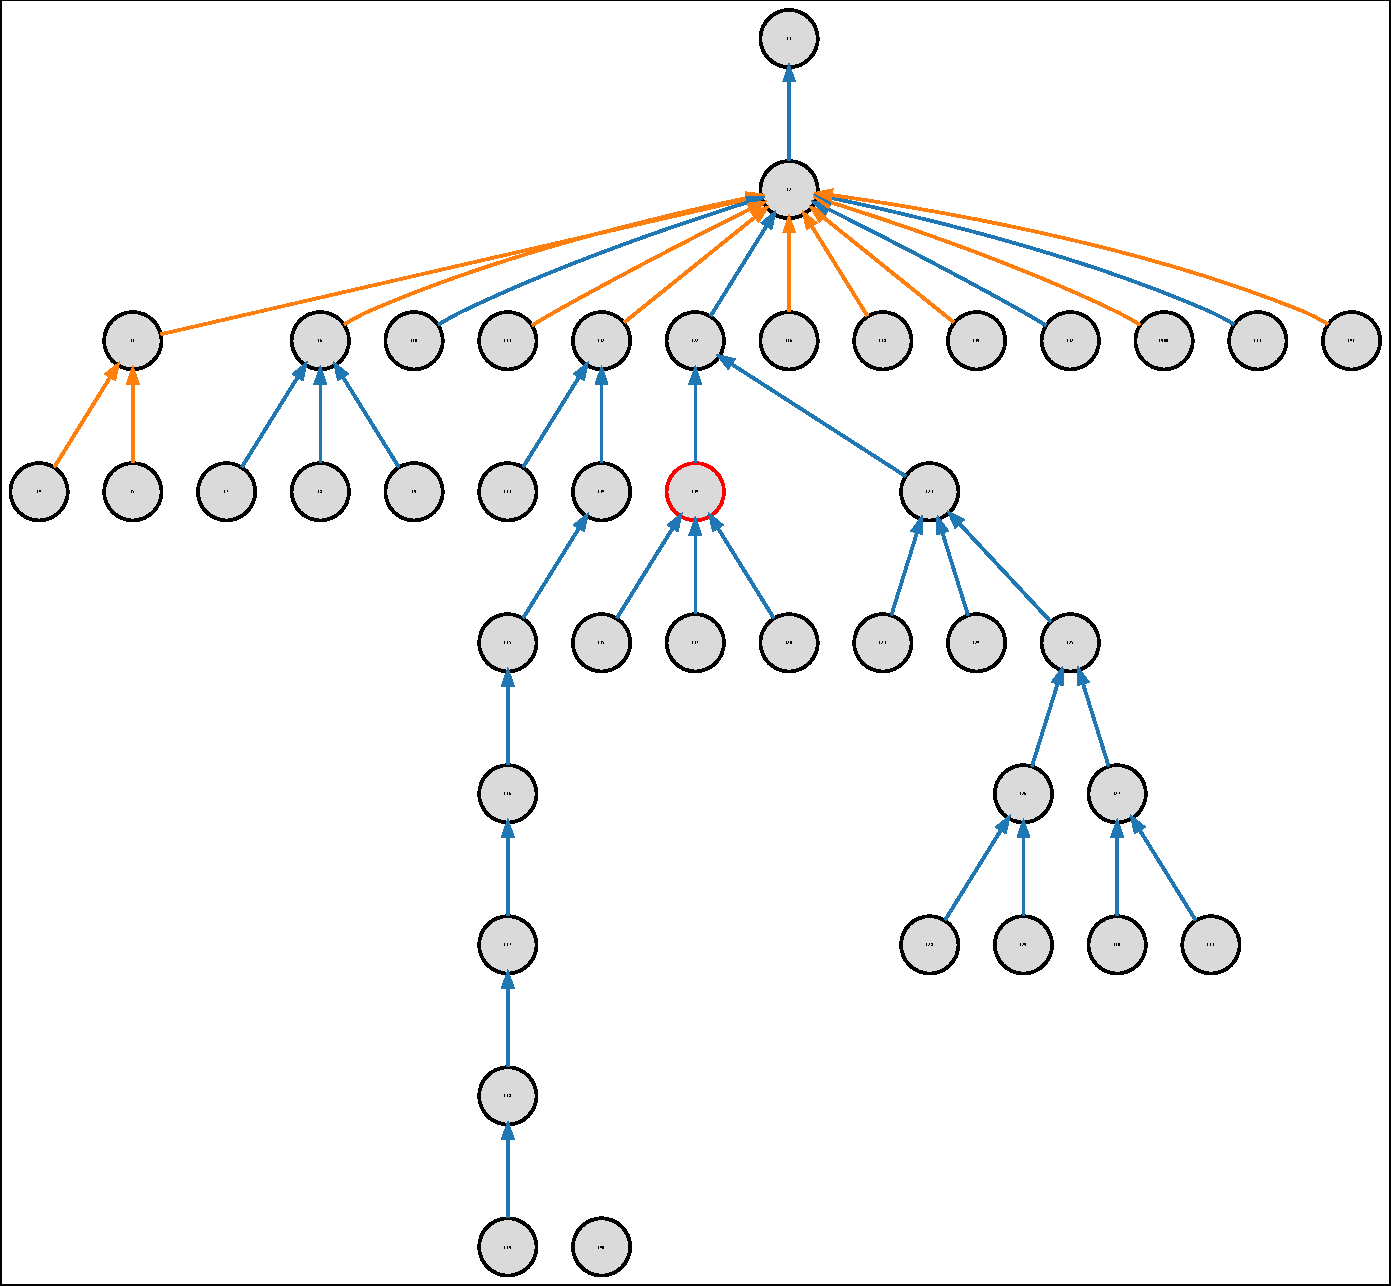
\includegraphics[trim=0mm 0mm 235mm 218mm, clip,width=50mm]{img/erk-graph-builtins}
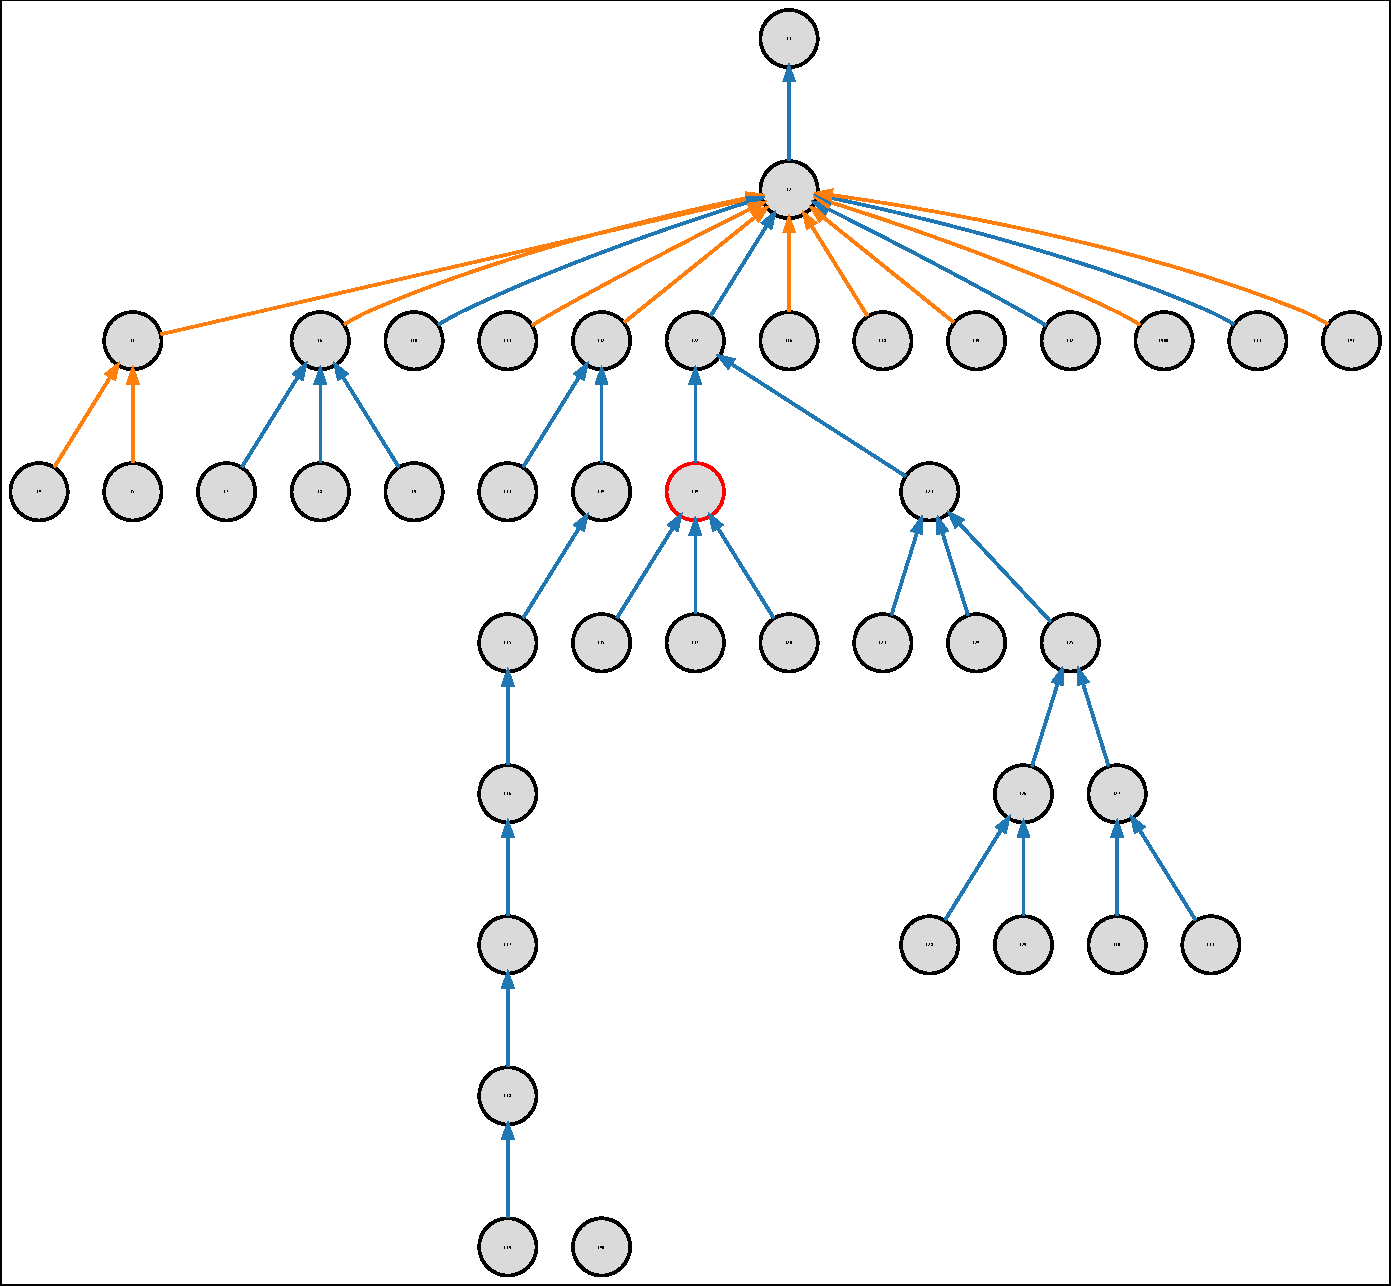
\includegraphics[clip,width=45mm]{img/erk-graph-builtins}
}
\end{textblock*}

\begin{textblock*}{40mm}[0.,0.](10mm,26mm)
\visible<3>{
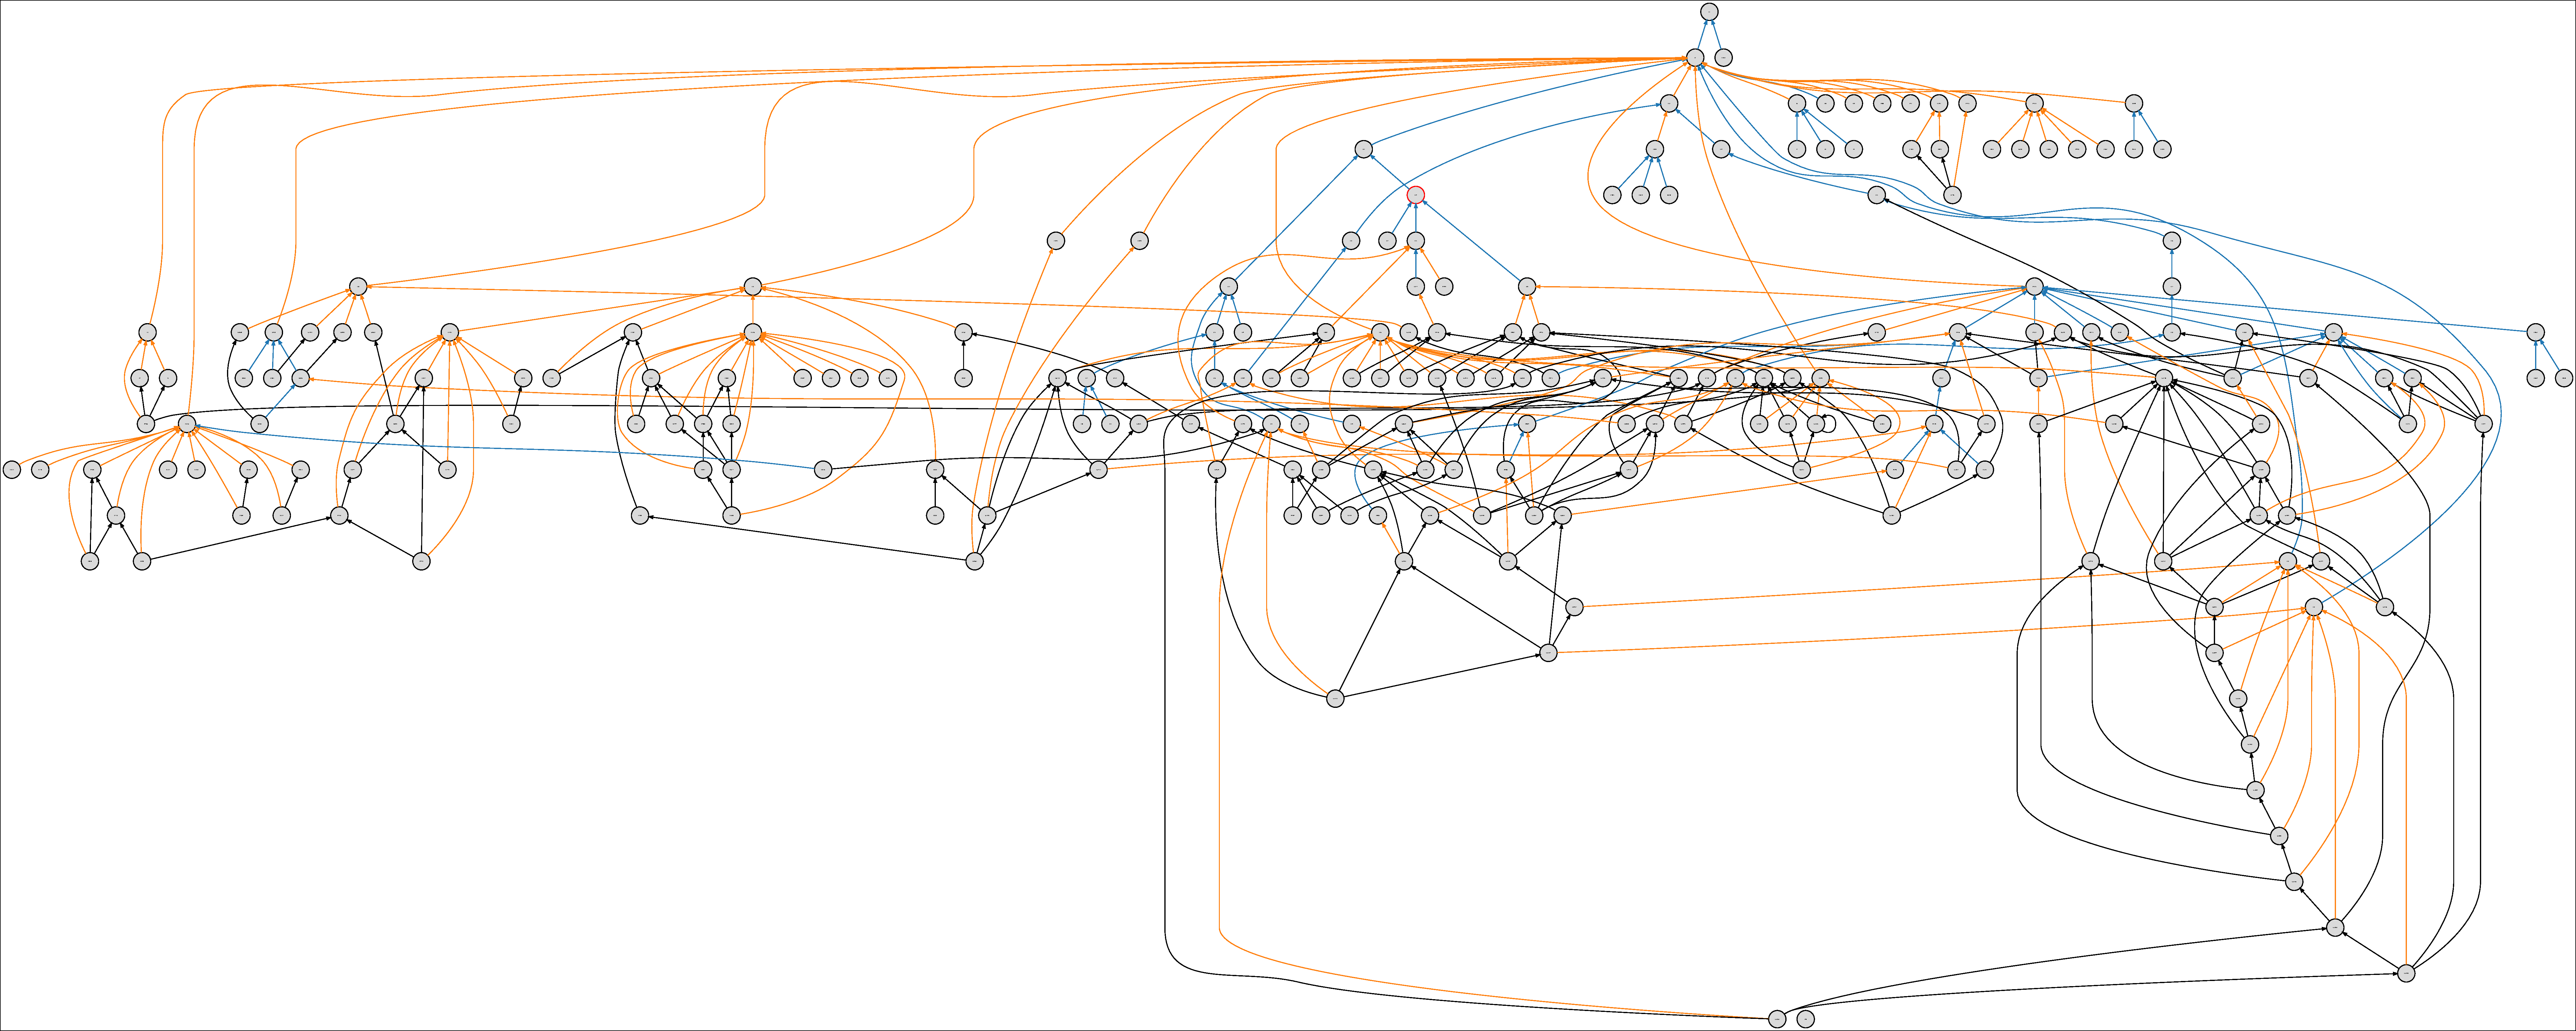
\includegraphics[width=135mm]{img/erk-graph-all.pdf}
}
\end{textblock*}

\pause
\pause
\pause

\medskip
\only<4->{
\textbf{Bisherige Anwendung:}

Klassifikation von Enititäten im \textbf{A}utomatic \textbf{C}ontrol \textbf{K}nowledge \textbf{Rep}ository (ACKREP)

\smallskip
(Systemmodelle, Problembeschreibungen, Lösungsmethoden)

\pause
\smallskip
$\rightarrow$ Ermöglicht SPARQL-Suche\\
(z.\,B. exakt E-Z-linearisierbare Modelle mit $n > 3$)


\begin{textblock*}{40mm}[0.,0.](97mm,39mm)
\visible<4->{
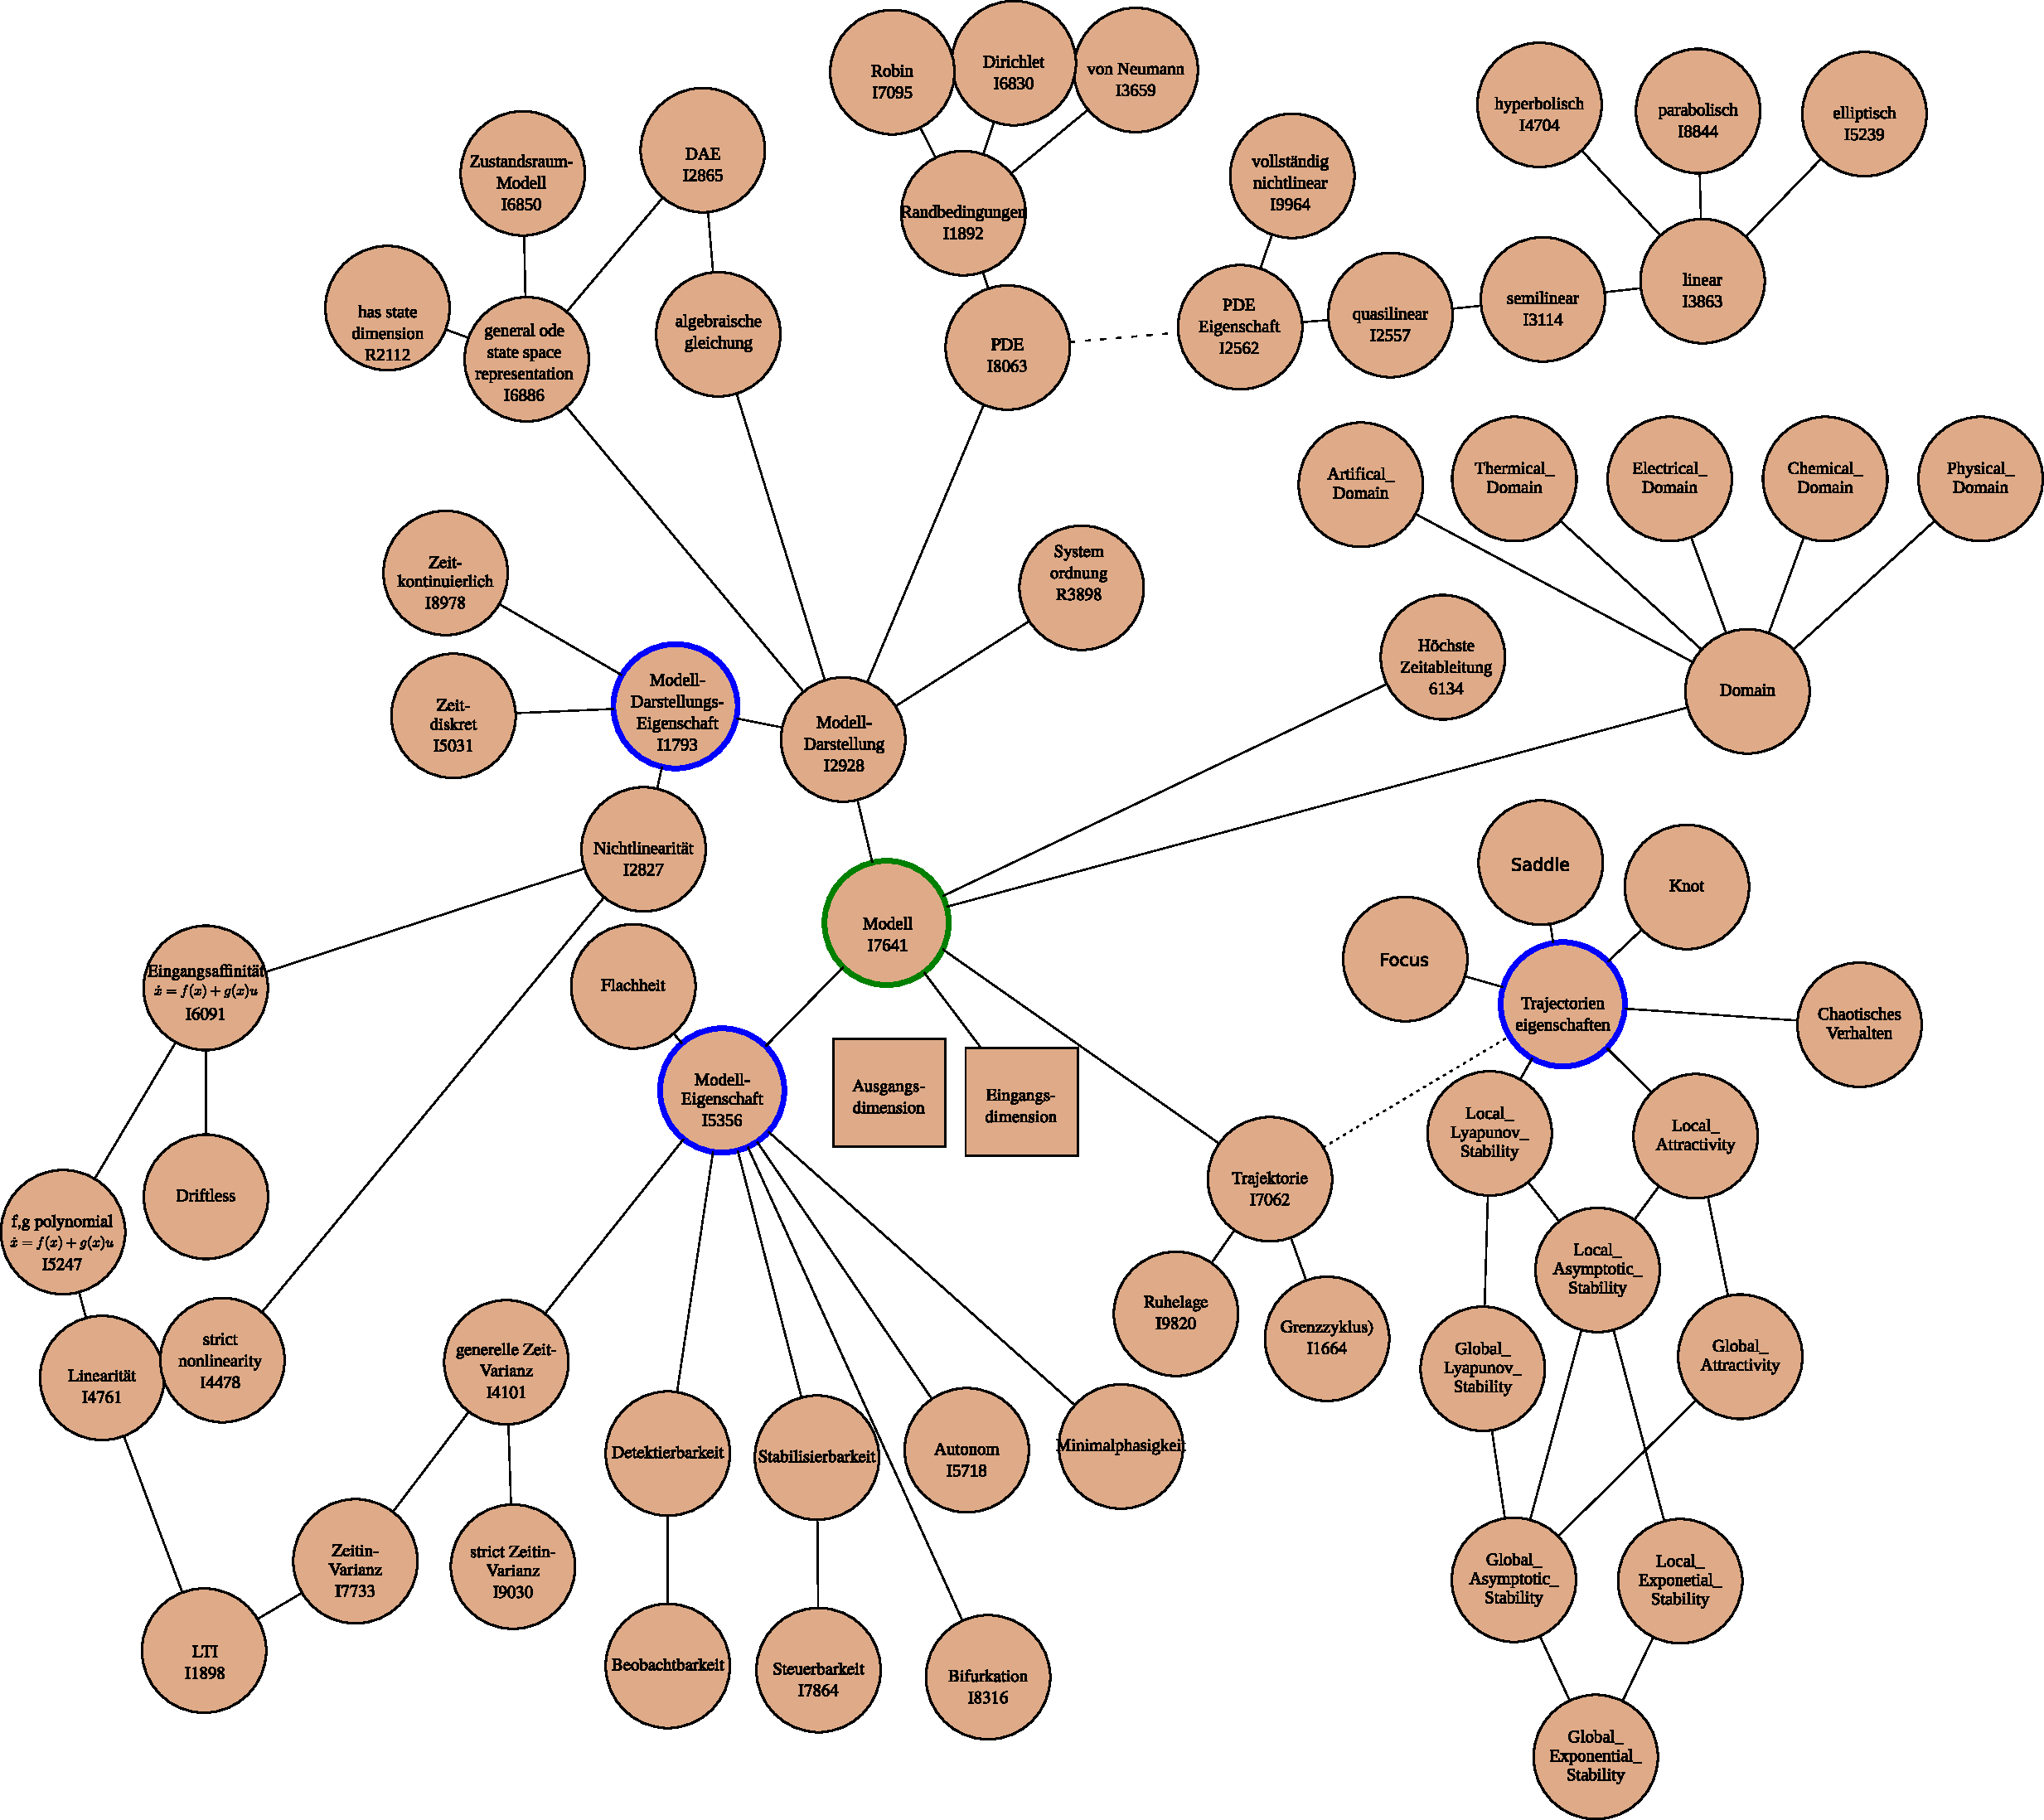
\includegraphics[width=50mm]{img/model_classification.pdf}
}
\end{textblock*}



\pause

\medskip
\bigskip
\textbf{Mögliche zukünftige Anwendungen}

\begin{itemize}
 \item (Autom.) Klassifikation von Veröffentlichungen\\
 Denkbar: bis auf Satz- bzw. Gleichungsebene.
 
 \item Assistenzsoftware für Reglerentwurf
 
\end{itemize}

$\rightarrow$ Wissenstransfer

}

\end{frame}
%%%%%%%%%%%%%%%%%%%%%%%%%%%%%%%%%%%%%%%%%%%%%%%%%%%%%%%%%%%%%%%%%%%%%%%%%%%%%%%%


\againframe<4>{gl1}


%%%%%%%%%%%%%%%%%%%%%%%%%%%%%%%%%%%%%%%%%%%%%%%%%%%%%%%%%%%%%%%%%%%%%%%%%%%%%%%%
  
\begin{frame}[t,fragile,label=zf1]{\large Zusammenfassung {\color<1-3>{mygray}und Diskussion}}
\begin{itemize}

 \item 
Formale Wissensrepräsentation potenziell nützlich für Wissenstransfer

\pause
\medskip
 \item 
Für Regelungstheorie existiert noch keine etablierte Technologie

\pause
\medskip
 \item 
Experimenteller Vorschlag: ERK + OCSE (Code und Daten sind Open Source)\\[3mm] \hfill {\Large $\rightarrow$ \url{https://ackrep.org}}
\end{itemize}

\pause
\bigskip
{\large \textbf{Diskussion} (offene Fragen)}

\begin{itemize}
 \item Grundsätzliche Tauglichkeit?

 \medskip
 \item (Automatisierte) Qualitätssicherung?
 
 \medskip
 \item Wissensintegration als sozialer Prozess?
\end{itemize}


\bigskip
\pause
$\rightarrow$ Herzliche Einladung zur Kollaboration



\begin{textblock*}{40mm}[0.,0.](110mm,45mm)
\visible<5->{
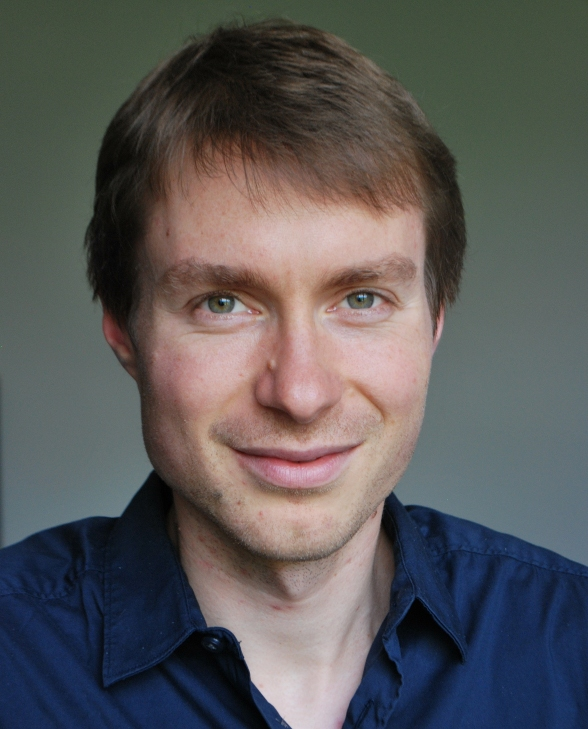
\includegraphics[width=23mm]{img/portrait-foto-knoll.jpg}\\[1mm]

{\tiny \texttt{Carsten.Knoll@tu-dresden.de}}
}
\end{textblock*}




\end{frame}

\begin{frame}[fragile,label=zf2]{~}
\begin{center}
{\huge \textbf{Ergänzungsfolien}} 
\end{center}

\end{frame}



\backupbegin




\begin{frame}[t,fragile,label=wr8]{\large Wissensrepräsentation (5): \underline{O}pen \underline{R}esearch \underline{K}nowledge \underline{G}raph}

  \begin{itemize}
  \item Projekt der Technischen Informationsbibliothek (TIB) Hannover
%   ist die Deutsche Zentrale Fachbibliothek für Technik sowie Architektur, Chemie, Informatik, Mathematik und Physik mit Sitz in Hannover. 
   \item Selbstbeschreibung: \textit{Infrastruktur-Dienst zur Sammlung von akademischem Wissen in maschinenverarbeitbarer Form.} 
%    [and] thus enabling new possibilities for scholarly knowledge curation, publication and processing
  \end{itemize}

  \pause
  \medskip
Grundlegendes Schema:
  
  
  \begin{textblock*}{40mm}[0.,0.](12mm,40mm)
\visible<2->{
  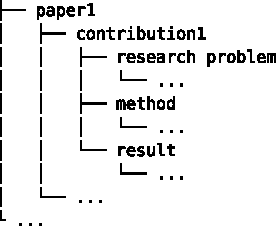
\includegraphics[width=40mm]{img/listing1.pdf}
}
\end{textblock*}

\begin{textblock*}{40mm}[0.,0.](55mm,30mm)
\visible<3>{
  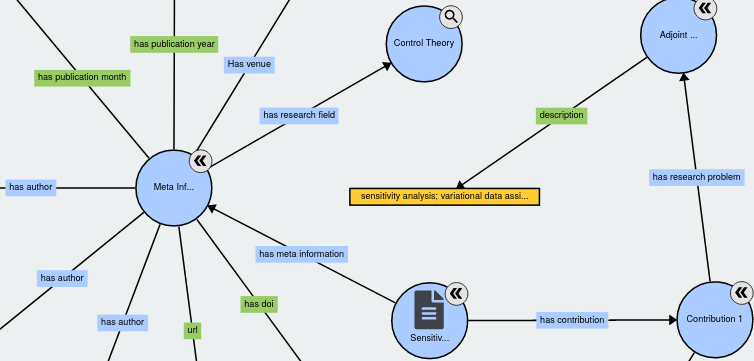
\includegraphics[width=100mm]{img/paper-graph-view.png}
}
\end{textblock*}
  

\begin{textblock*}{100mm}[0.,0.](65mm,30mm)
\visible<4>{
\begin{center}
 
Repräsentanz der Regelungstheorie:\\[1mm]

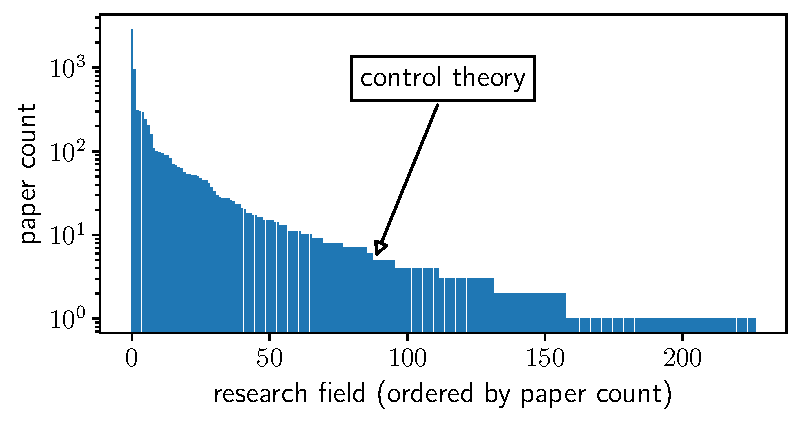
\includegraphics[width=78mm]{img/researchfield_ordered_by_paper-hist}
\end{center}
}
\end{textblock*}
  



\begin{textblock*}{130mm}[0.,0.](12mm,75mm)
\visible<5>{
$\rightarrow$ Bisher nur „grobe“ Wissensrepräsentation möglich/üblich
}
\end{textblock*}
  
  
\end{frame}
%%%%%%%%%%%%%%%%%%%%%%%%%%%%%%%%%%%%%%%%%%%%%%%%%%%%%%%%%%%%%%%%%%%%%%%%%%%%%%%%

\againframe<6->{wr7}

%%%%%%%%%%%%%%%%%%%%%%%%%%%%%%%%%%%%%%%%%%%%%%%%%%%%%%%%%%%%%%%%%%%%%%%%%%%%%%%%



\backupend





% \begin{frame}[fragile,label=test0]
% 
% 
% \lstset{
% % emph={proc,retp,endp,local}, emphstyle={\color{blue}\textbf},
% literate={./}{{{\color{red}./}}}2 {=}{{{\color{red}=}}}1
% }
% 
% \begin{lstlisting}
% proc(1) = tdist(n,v);
% a=b
% local x, z, z2, u, t;
% x=rndn(n,1); 
% z=rndn(n,v);
% z2=z.^2; 
% t=x./((U./v)^(1/2));
% retp(t);
% endp;
% \end{lstlisting}
% 
% 
% \end{frame}
% \begin{frame}[fragile,label=test1]
% 
% 
% 
% \begin{pythoncode}
% I400 = p.create_item(
%     R1__has_label="transitivity of R17__is_subproperty_of",
%     R4__is_instance_of=p.I41["semantic rule"],
% )
% \end{pythoncode}
% \pause
% 
% \begin{pythoncode}
% a = effi = p.create_item(
%     I1234__text="World",
% )
% f"Hello {a}"  # use variables
% \end{pythoncode}
% 
% test
% 
% \end{frame}
%  

\end{document}


